% ==============================================
% CHAPTER: SOFTWARE DESIGN
% ==============================================
\chapter{Software Design}

%===========================================================
\section{Introduction to Software Design}
%===========================================================

This chapter presents the detailed software design of the Lets Go Ride Sharing App ride-sharing and recommendation system. It translates the requirements identified in Chapter 3 into structured architectural, behavioral, and data models. The purpose of this chapter is to provide a clear blueprint for system implementation, ensuring maintainability, scalability, and modular development.

The design follows Object-Oriented Design (OOD) principles and implements a hybrid architecture combining Multi-Tier and Model-View-Controller (MVC) patterns. This chapter includes architectural design, UML models (class, sequence, state, activity diagrams), data flow models, database design, and detailed algorithms for core functionalities including ML-based ride recommendations, route ETA calculation, and SOS escalation logic.

%===========================================================
\section{Design Methodology and Software Process Model}
%===========================================================

\subsection{Design Methodology}

The design process embraced in the Lets Go Ride Sharing App system is Object-Oriented Design (OOD). The system has various real-world objects including Passenger, Driver, Ride, Vehicle, Booking, Payment, and Route with their own attributes and behaviours. Object-oriented modeling is the best method to map these real-world concepts to software components.

\subsubsection{Reasons behind the use of Object-Oriented Design (OOD)}

\begin{itemize}
    \item \textbf{Inherent Recreation of Real-Life Objects:} OOD enables the project to represent core domain objects, including users, vehicles, rides, and trip requests, as classes having attributes and methods. This enhances the clarity of concepts and aligns with the domain outlined in the SRS.
    
    \item \textbf{Reusability and Extensibility:} The application includes multiple modules (Authentication, Ride Matches, ML Recommendations, SOS Handling, Chat, Notifications) allowing OOD to achieve reuse via inheritance, interfaces, and composition. New features (e.g., corporate rides, scheduled rides) can be added without rewriting core modules.
    
    \item \textbf{Encapsulation and Modularity:} The system is built with the MVC (MTV) pattern of Django with models, views, controllers and services being defined as separate modules. Encapsulation ensures that each module is responsible for its own task.
    
    \item \textbf{Conformity with Multi-Tier Architecture:} Object-oriented modules can be distributed across layers since the application is based on the multi-tier architecture (Client, Backend Servers, Database, External Services).
    
    \item \textbf{Support for Scalability:} Horizontal scaling is facilitated with multiple backend servers, all running the same OOP-based services. Classes like BookingManager, RideManager, VerificationManager, and MLService separate complex logic into manageable units.
    
    \item \textbf{Simplified Maintenance:} Classes separate complex logic into single, manageable units which are easy to debug and update.
\end{itemize}

The design follows key software engineering principles including SOLID (Single Responsibility, Open-Closed, Liskov Substitution, Interface Segregation, Dependency Inversion), DRY (Don't Repeat Yourself), and Separation of Concerns.

\subsection{Software Process Model}

The project follows the \textbf{Agile Incremental Development Model} with Scrum-like iterations.

\subsubsection{Justification for Using Agile/Scrum}

\begin{itemize}
    \item \textbf{Rapid Requirement Evolution:} Ride-sharing systems have evolving requirements such as new safety rules, changes in verification flows, and improvements in rider-driver matching. Agile enables the team to accommodate changes with high frequency while retaining stability.
    
    \item \textbf{Modular and Incremental Delivery:} The system was built in significant increments:
    \begin{itemize}
        \item Increment 1: User signup/login
        \item Increment 2: Ride creation and search
        \item Increment 3: Driver acceptance flow
        \item Increment 4: Live tracking \& periodic HTTP updates
        \item Increment 5: SOS, dispute, notifications
        \item Increment 6: ML recommendations
    \end{itemize}
    This aligns perfectly with the incremental approach.
    
    \item \textbf{Ongoing Feedback of End Users:} Ride-sharing applications need to be tested by actual users to confirm usability, map accuracy, and ride matching quality. Agile cycles enabled feedback from users on early releases.
    
    \item \textbf{Concurrent Development of Subsystems:} Multiple modules including Mobile App, Backend API, External Services, Chatbot, and ML Recommendation Engine were worked on simultaneously based on iterative sprints.
    
    \item \textbf{Reduced Project Risk:} Features were developed, constructed, and tested in bursts, minimizing the risk of last-minute failures.
    
    \item \textbf{Fit for Academic Projects:} Agile offers flexibility of documentation while allowing structured artifacts (SRS, SDD, UML models).
\end{itemize}

Testing and validation were integrated into each sprint through continuous integration, unit testing, and user acceptance testing at the end of each increment.

%===========================================================
\section{System Overview}
%===========================================================

This section provides a high-level overview of system components and interactions with external entities.

\subsection{External Actors}

\begin{itemize}
    \item \textbf{Passenger (Mobile App):} Requests rides, browses available options, tracks drivers, and completes trips.
    \item \textbf{Driver (Mobile App):} Shows availability, accepts rides, shares live location, and completes trips.
    \item \textbf{Administrator (Web Portal):} Monitors the system, verifies users, and manages disputes.
\end{itemize}

\subsection{External Services}

\begin{itemize}
    \item \textbf{Map API (OpenStreetMap/OSRM):} Route calculation, reverse geocoding, and ETA estimation.
    \item \textbf{Notification Services (Supabase/FCM):} Sends real-time notifications for ride requests, acceptances, and SOS alerts.
    \item \textbf{Machine Learning Service:} Recommends best-fitting rides to passengers based on past information.
    \item \textbf{Chatbot/AI Assistant:} Automated support for frequently asked questions.
    \item \textbf{Storage Service:} Manages profile pictures, license files, and verification documents.
\end{itemize}

\subsection{Backend (Django MVC + JSON APIs)}

The central component of the system fulfills:
\begin{itemize}
    \item Ride matching logic
    \item Booking and cancellation
    \item Location updates via periodic HTTP requests
    \item Profile and document verification
    \item ML-based recommendation calls
    \item SOS escalation and dispute management
    \item Managing communication with drivers and passengers
\end{itemize}

\subsection{Database (PostgreSQL)}

Stores:
\begin{itemize}
    \item Passenger/Driver profiles
    \item Documents and verification states
    \item Ride requests and bookings
    \item Payment and trip summaries
    \item Dispute logs
    \item Chat history
\end{itemize}

\subsection{Context Diagram}

\begin{figure}[htbp]
\centering
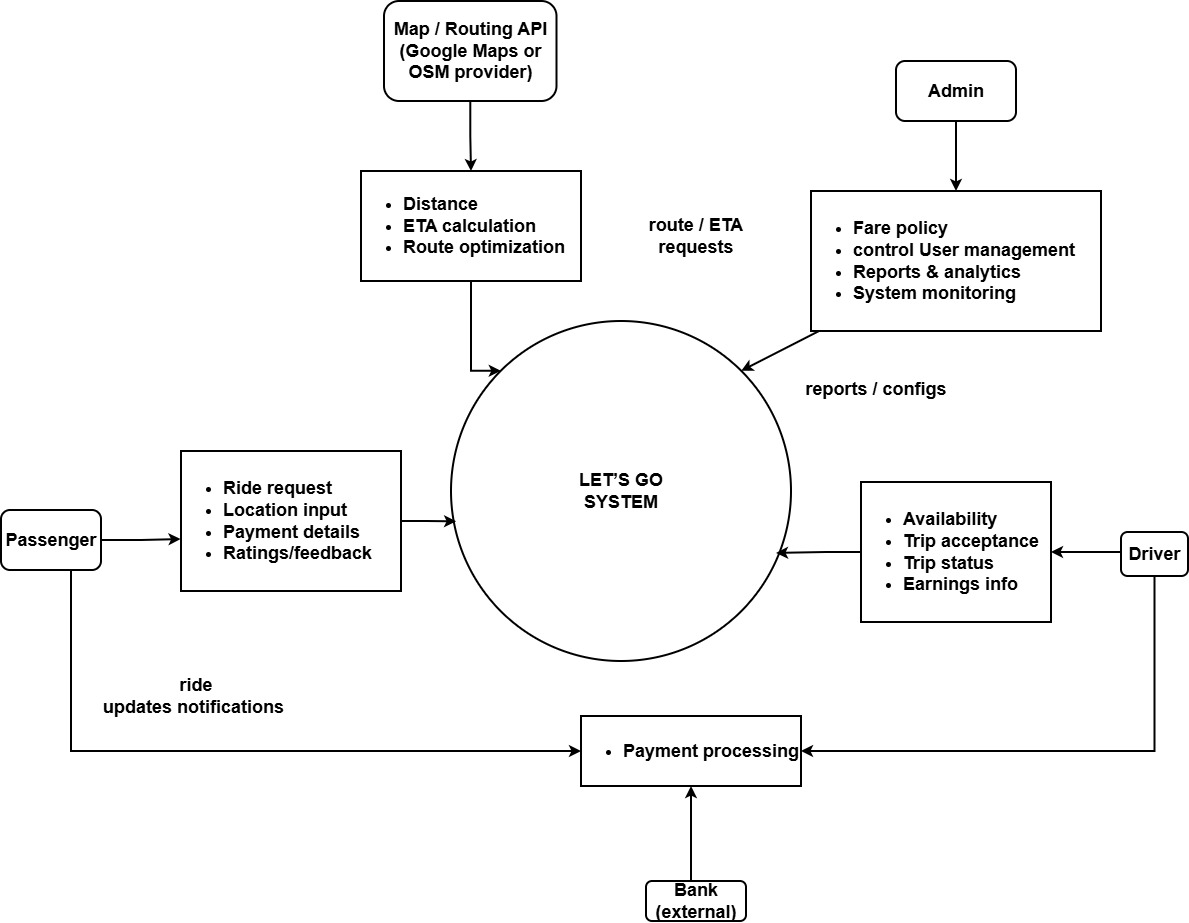
\includegraphics[width=0.9\textwidth,keepaspectratio,height=0.8\textheight]{assets/context Diagram-Page-2.jpg}
\caption{Context Diagram showing system boundary and interactions with external actors and services}
\label{fig:context}
\end{figure}

The context diagram illustrates the Lets Go Ride Sharing App system boundary and its interactions with external entities including Passengers, Drivers, Administrators, and third-party services (Map API, Notification Service, ML Service, Chatbot, Storage). Data flows represent ride requests, location updates, notifications, and document transfers.

%===========================================================
\section{Architectural Design}
%===========================================================

The Lets Go Ride Sharing App system is built under a hybrid architectural style consisting of two broad paradigms:
1. Multi-Tier Architecture for the overall system structure
2. Model-View-Controller (MVC) internally in the backend through Django framework

The combination offers separation of concerns, scalability, maintainability, and distributed deployment over several servers.

\subsection{Architecture Style (MVC + Multi-tier)}

\subsubsection{MVC Architecture (within Django backend servers)}

\begin{table}[htbp]
\centering
\caption{Backend MVC Structure}
\renewcommand{\arraystretch}{1.3}
\begin{tabularx}{\textwidth}{|X|X|X|}
\hline
\textbf{Layer} & \textbf{Component} & \textbf{Description} \\
\hline
Model & Django Models & Data representation and database ORM mappings \\
\hline
View & Templates / API serializers & Presentation logic for admin or API responses \\
\hline
Controller & Views & Request handling \& business logic \\
\hline
\end{tabularx}
\end{table}

Services are separated as independent modules:
\begin{itemize}
    \item AuthService
    \item RideManager
    \item VerificationManager
    \item NotificationService
    \item MLService
    \item ChatService
\end{itemize}
This ensures modularity, testability, and easier scalability.

\subsection{High-Level System Components}

The system is composed of:
\begin{itemize}
    \item \textbf{Client Layer:} Mobile apps (Passenger/Driver), Admin dashboard (web)
    \item \textbf{Application Layer:} Multiple identical backend servers running Django with JSON-based APIs for core features; mobile clients implement real-time behavior using periodic HTTP updates
    \item \textbf{External Services Layer:} Map API, Notifications (Supabase/FCM), Storage, ML recommendations, Chatbot
    \item \textbf{Data Layer:} PostgreSQL relational database, centralized and transaction-safe
\end{itemize}

\subsection{Multi-Tier Deployment Architecture}

\subsubsection{Tier 1 - Client Layer}
\begin{itemize}
    \item Flutter-based mobile applications for passengers and drivers
    \item HTML/CSS/JavaScript web-based admin dashboard
\end{itemize}

\subsubsection{Tier 2 - Application Layer}
\begin{itemize}
    \item Django backend servers with JSON-based APIs for authentication, rides, bookings, payments, safety, and administration
    \item Real-time behavior is achieved on the clients using periodic HTTP updates and push notifications where available
\end{itemize}

\subsubsection{Tier 3 - External Services Layer}
\begin{itemize}
    \item Map Service (OSRM/OpenStreetMap): Route calculation, distance, ETA
    \item Notification Service (FCM, SMS, Email)
    \item ML Recommendation Service: TF-IDF based ride recommendations
    \item Chatbot Service: Generative AI for FAQ support
    \item Storage Service: Document and image management
\end{itemize}

\subsubsection{Tier 4 - Data Layer}
\begin{itemize}
    \item PostgreSQL (Supabase) for transactional data
    \item Geospatial computations are handled in application logic for distance and route summaries
\end{itemize}

\subsection{External Services Integration}

Backend servers interface with external services through well-defined REST APIs with token-based authentication and fault-tolerant retry mechanisms.

\subsubsection{Map Service}
\begin{itemize}
    \item Reverse geocoding
    \item Route calculations
    \item Distance and ETA estimation
\end{itemize}

\subsubsection{Notification Service}
\begin{itemize}
    \item Push notifications via FCM
    \item Alerts for ride request, driver acceptance, SOS
\end{itemize}

\subsubsection{ML Recommendation Service}
\begin{itemize}
    \item Receives ride request data
    \item Returns list of recommended rides
    \item Uses TF-IDF similarity
\end{itemize}

\subsubsection{Chatbot Service}
\begin{itemize}
    \item Provides automated FAQ responses
\end{itemize}

\subsubsection{Storage Service}
\begin{itemize}
    \item Uploading profile images
    \item Uploading verification documents
    \item Generating signed URLs
\end{itemize}

\subsection{Architecture Diagram}

The architecture diagram illustrates the four tiers: Client Layer (Mobile Apps, Admin Web), Application Layer (Django Backend with MVC and JSON APIs), External Services Layer (Map, Notifications, ML, Chatbot, Storage), and Data Layer (PostgreSQL). Arrows indicate data flow and API interactions between components.

\begin{figure}[H]
\centering
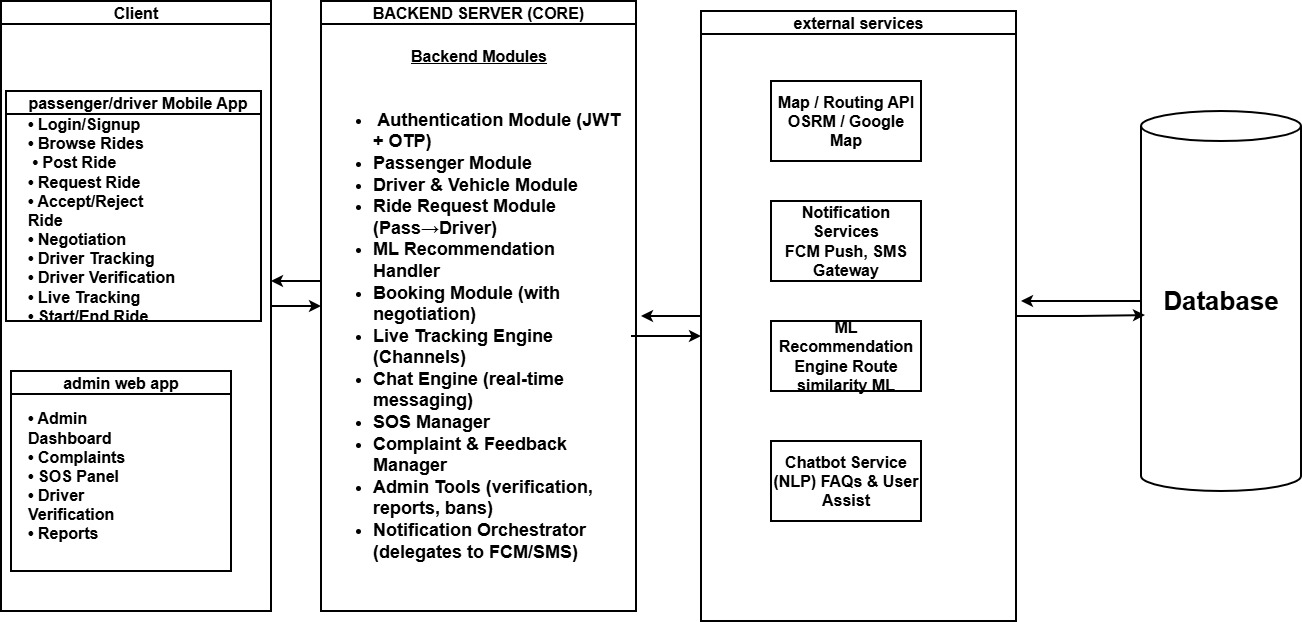
\includegraphics[width=0.9\textwidth,keepaspectratio,height=0.8\textheight]{assets/architecture.jpg}
\caption{High-level system architecture diagram showing multi-tier deployment and component interactions}
\label{fig:architecture}
\end{figure}

%===========================================================
\section{Design Models}
%===========================================================

This section presents detailed design models of the system. These models describe system behavior, structure, and interactions using UML diagrams. The models help developers understand system workflow before implementation.

%===========================================================
\subsection{Activity Diagrams}

Activity diagrams represent the workflow of different modules of the system. Each core module has a separate activity diagram showing user interaction, decision nodes, validation checks, and database/model interaction.

\subsubsection{Authentication \& Onboarding (Register, OTP, Admin verify)}

\begin{figure}[H]
\centering
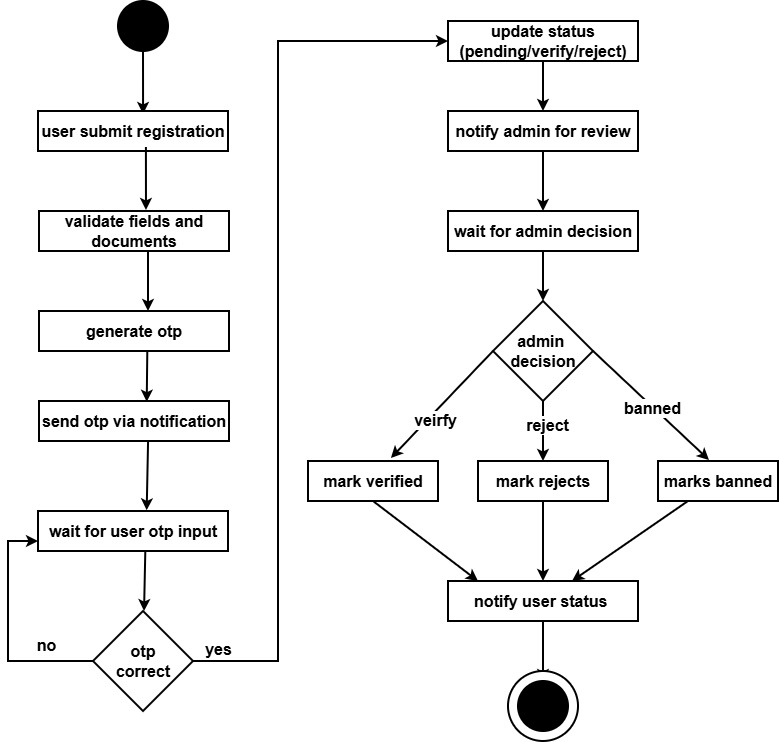
\includegraphics[width=0.8\textwidth,keepaspectratio,height=0.8\textheight]{assets/activity diagrams/activity_auth.jpg}
\caption{Activity Diagram - Authentication and Onboarding workflow}
\label{fig:activity_auth}
\end{figure}

This diagram illustrates the complete user registration and verification process: user enters details, uploads documents, receives OTP via email/SMS, verifies OTP, and awaits admin approval. Admin reviews documents and either verifies, rejects, or bans the user.

\clearpage

\subsubsection{Document Management (uploads \& verification)}

\begin{figure}[H]
\centering
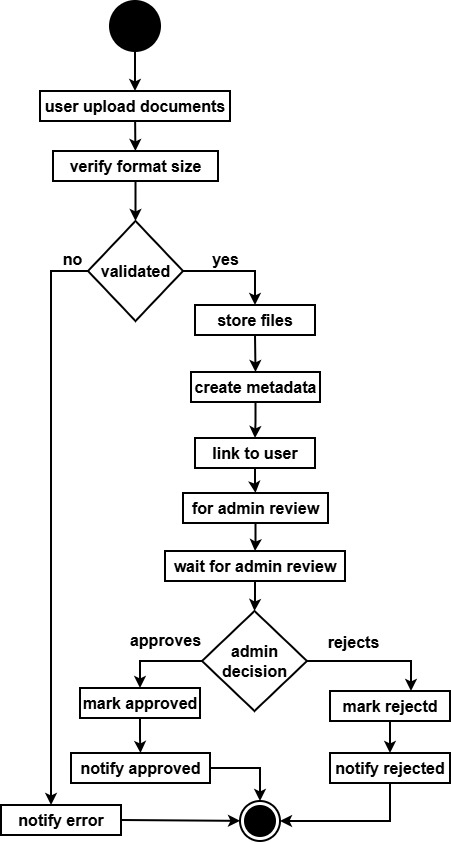
\includegraphics[width=0.6\textwidth,keepaspectratio,height=0.8\textheight]{assets/activity diagrams/activity_document.jpg}
\caption{Activity Diagram - Document Management workflow}
\label{fig:activity_document}
\end{figure}

Shows the process of document upload, validation (format/size), storage, and admin verification workflow including approval/rejection cycles.

\clearpage

\subsubsection{Vehicle Management (add/edit/delete vehicles)}

\begin{figure}[H]
\centering
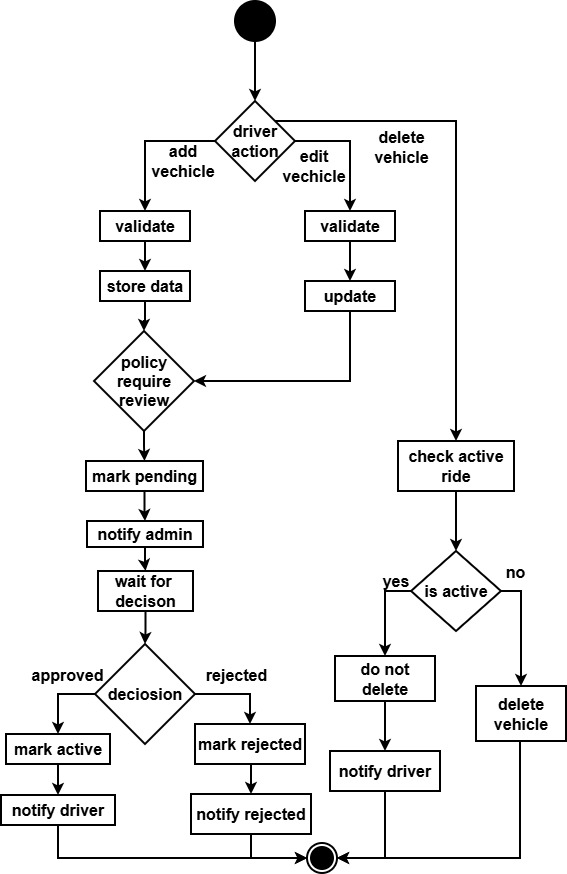
\includegraphics[width=0.8\textwidth,keepaspectratio,height=0.8\textheight]{assets/activity diagrams/module 3.jpg}
\caption{Activity Diagram - Vehicle Management workflow}
\label{fig:activity_vehicle}
\end{figure}

Depicts driver adding vehicle details, uploading images, system validation, and optional admin review for critical changes.

\clearpage

\subsubsection{Ride Management (create/edit/cancel, route \& stops)}

\begin{figure}[H]
\centering
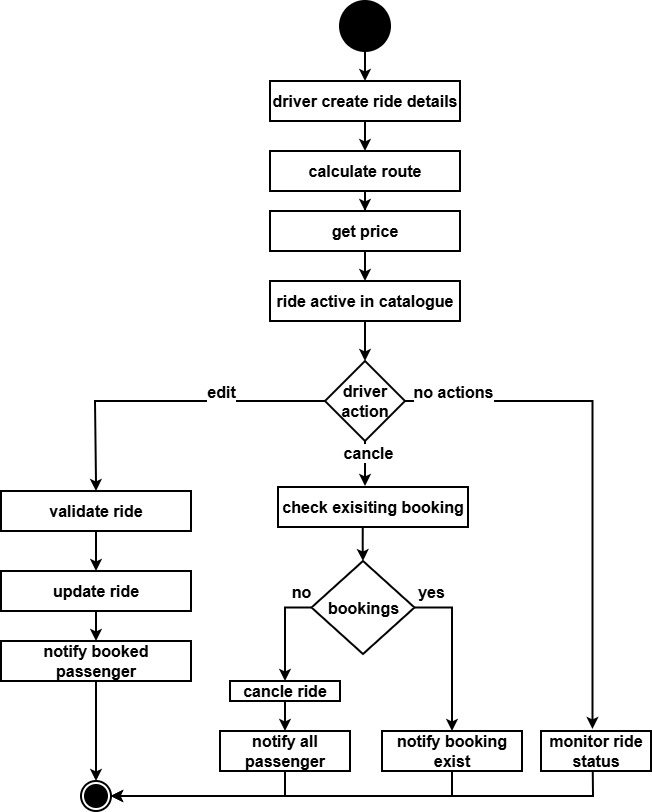
\includegraphics[width=0.8\textwidth,keepaspectratio,height=0.8\textheight]{assets/activity diagrams/module4.jpg}
\caption{Activity Diagram - Ride Management workflow}
\label{fig:activity_ride_mgmt}
\end{figure}

Illustrates driver creating a ride with map-based route editor, setting parameters (date/time, seats, gender preference, fare), validation, and publishing.

\clearpage

\subsubsection{Marketplace / Browse \& Search / Ride Details}

\begin{figure}[H]
\centering
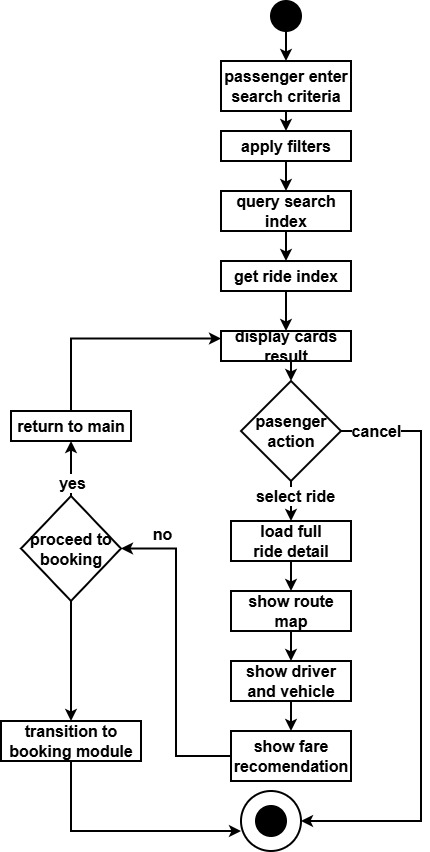
\includegraphics[width=0.8\textwidth,keepaspectratio,height=0.8\textheight]{assets/activity diagrams/module5.jpg}
\caption{Activity Diagram - Ride Browsing and Search workflow}
\label{fig:activity_browse}
\end{figure}

Shows passenger browsing available rides, applying filters, viewing ride cards with key information, and selecting a ride for detailed view.

\clearpage

\subsubsection{Booking \& Seat Management (select seats, lock seats)}

\begin{figure}[H]
\centering
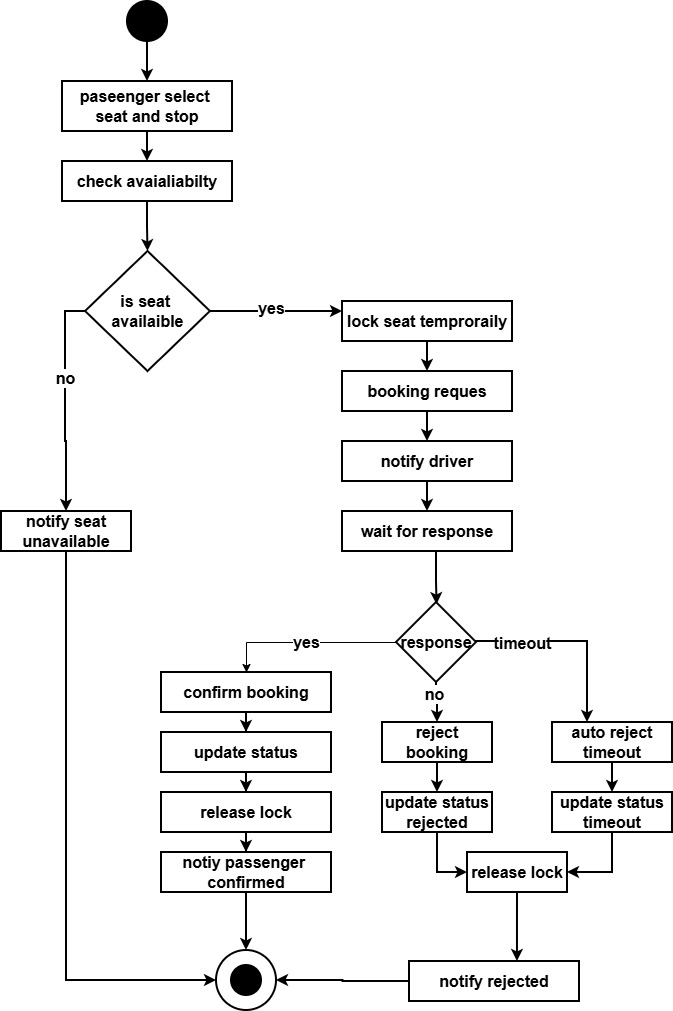
\includegraphics[width=0.8\textwidth,keepaspectratio,height=0.8\textheight]{assets/activity diagrams/module6.jpg}
\caption{Activity Diagram - Booking and Seat Management workflow}
\label{fig:activity_booking}
\end{figure}

Depicts passenger selecting pickup/drop stops, choosing seats (gender-based), special requests, fare calculation, seat locking, and driver acceptance/rejection.

\clearpage

\subsubsection{Post-Booking Chat / Messaging \& Broadcast}

\begin{figure}[H]
\centering
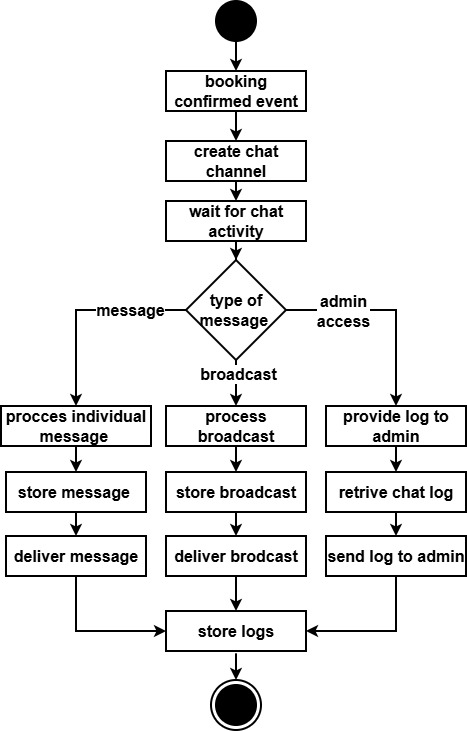
\includegraphics[width=0.8\textwidth,keepaspectratio,height=0.8\textheight]{assets/activity diagrams/module7.jpg}
\caption{Activity Diagram - Post-Booking Chat and Broadcast workflow}
\label{fig:activity_chat}
\end{figure}

Illustrates one-to-one messaging between driver and passengers, and driver broadcast to selected passengers.

\clearpage

\subsubsection{Scheduler / Pre-Ride Reminders \& Permission Prompt}

\begin{figure}[H]
\centering
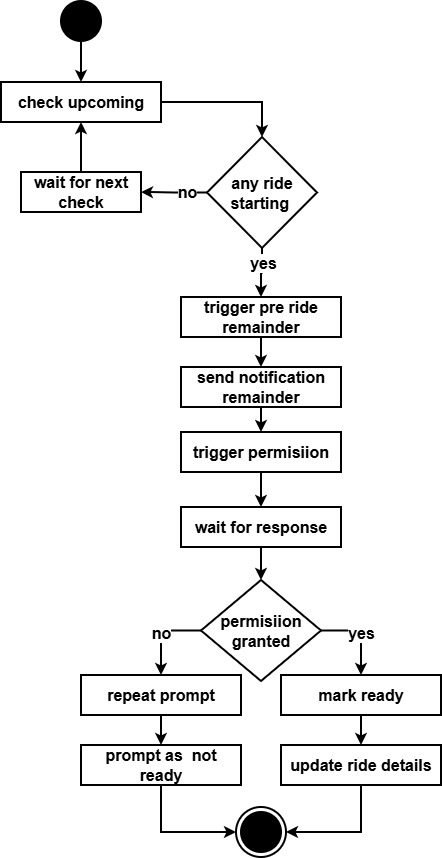
\includegraphics[width=0.8\textwidth,keepaspectratio,height=0.8\textheight]{assets/activity diagrams/module8.jpg}
\caption{Activity Diagram - Pre-Ride Reminders workflow}
\label{fig:activity_reminder}
\end{figure}

Shows scheduled reminders sent to driver and passengers, permission prompts, and readiness confirmation.

\clearpage

\subsubsection{Live Tracking \& Pickup Code (Start Ride / geofence)}

\begin{figure}[H]
\centering
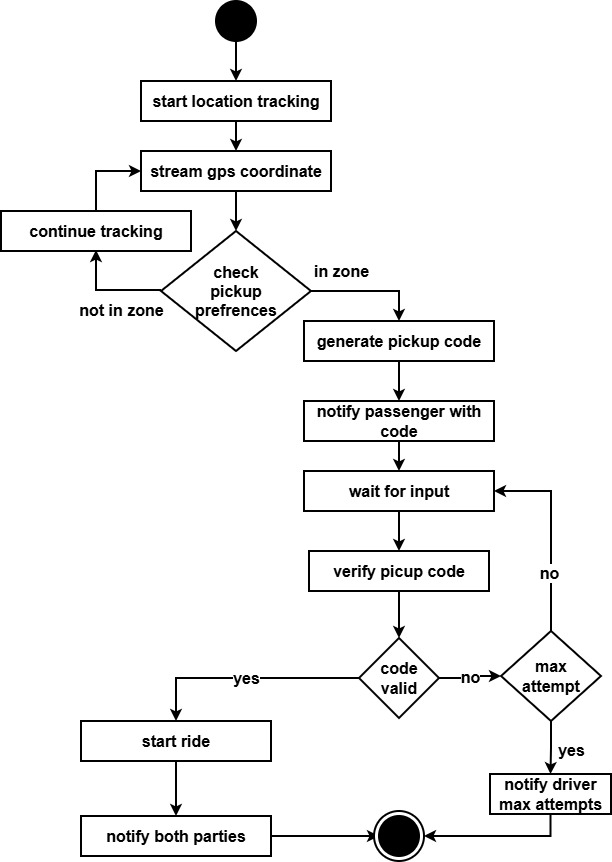
\includegraphics[width=0.8\textwidth,keepaspectratio,height=0.8\textheight]{assets/activity diagrams/module9.jpg}
\caption{Activity Diagram - Live Tracking and Pickup Code workflow}
\label{fig:activity_tracking}
\end{figure}

Depicts driver within geofence generating pickup code, passenger entering code, verification, and ride start.

\clearpage

\subsubsection{Payment \& Manual Payment Confirmation (cash / QR / bank transfer)}

\begin{figure}[H]
\centering
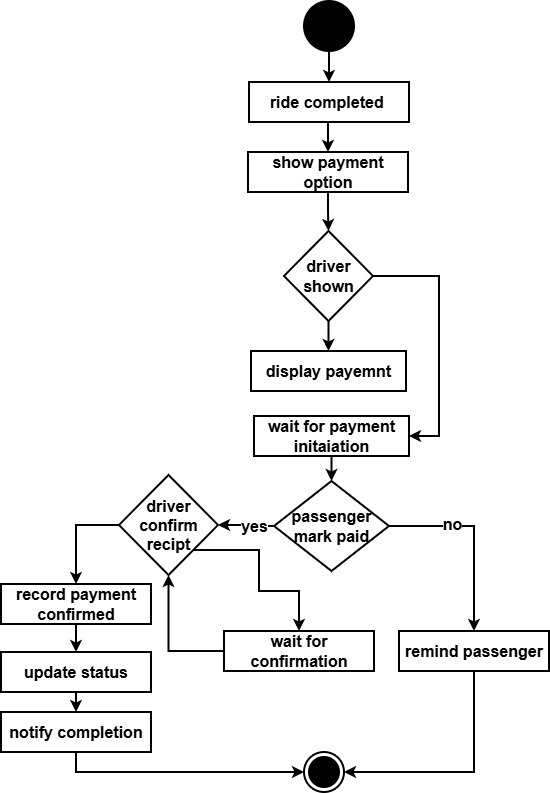
\includegraphics[width=0.8\textwidth,keepaspectratio,height=0.8\textheight]{assets/activity diagrams/module10.jpg}
\caption{Activity Diagram - Manual Payment Confirmation workflow}
\label{fig:activity_payment}
\end{figure}

Illustrates passenger marking reached, viewing driver bank details/QR, making payment, marking paid, and driver confirming receipt.

\clearpage

\subsubsection{Ratings \& Completion Workflow (mark reached, complete, rating)}

\begin{figure}[H]
\centering
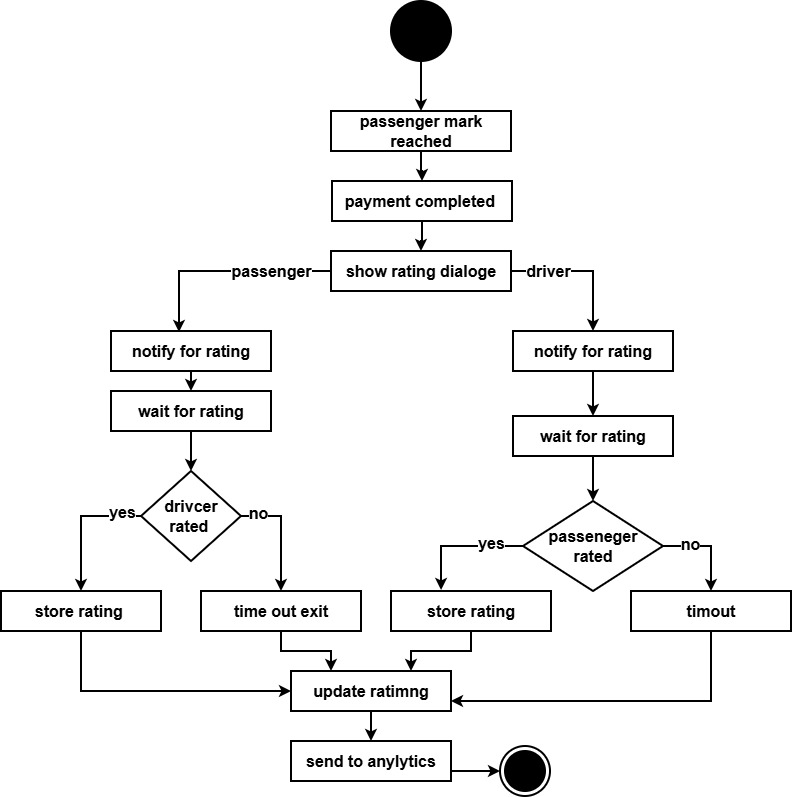
\includegraphics[width=0.8\textwidth,keepaspectratio,height=0.8\textheight]{assets/activity diagrams/module11.jpg}
\caption{Activity Diagram - Ratings and Completion workflow}
\label{fig:activity_rating}
\end{figure}

Shows passenger marking reached, rating prompt, driver marking complete, and mutual rating submission.

\clearpage

\subsubsection{SOS / Emergency \& Incident Management}

\begin{figure}[H]
\centering

\includegraphics[width=0.8\textwidth,keepaspectratio,height=0.8\textheight]{assets/activity diagrams/module 12.jpg}
\caption{Activity Diagram - SOS and Emergency workflow}
\label{fig:activity_sos}
\end{figure}

Depicts SOS trigger, immediate notifications to emergency contacts and admin, escalation timers, and incident resolution.

\clearpage

\subsubsection{Dispute Management \& Admin Dashboard (view \& resolve disputes)}

\begin{figure}[H]
\centering
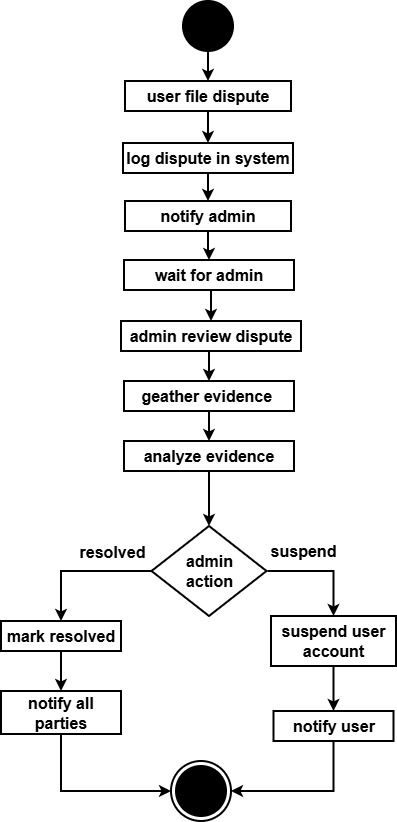
\includegraphics[width=0.8\textwidth,keepaspectratio,height=0.8\textheight]{assets/activity diagrams/module 13.jpg}
\caption{Activity Diagram - Dispute Management workflow}
\label{fig:activity_dispute}
\end{figure}

Illustrates user filing dispute, admin viewing evidence (chat logs, GPS traces), making resolution decision, and notifying parties.

\clearpage


%===========================================================
\subsection{Class Diagram}

The class diagram represents the static structure of the system by showing entities, their attributes, methods, and their relationships (association, aggregation, composition, inheritance). This diagram demonstrates encapsulation, inheritance, and associations as required by the object-oriented design methodology.

\begin{figure}[H]
\centering
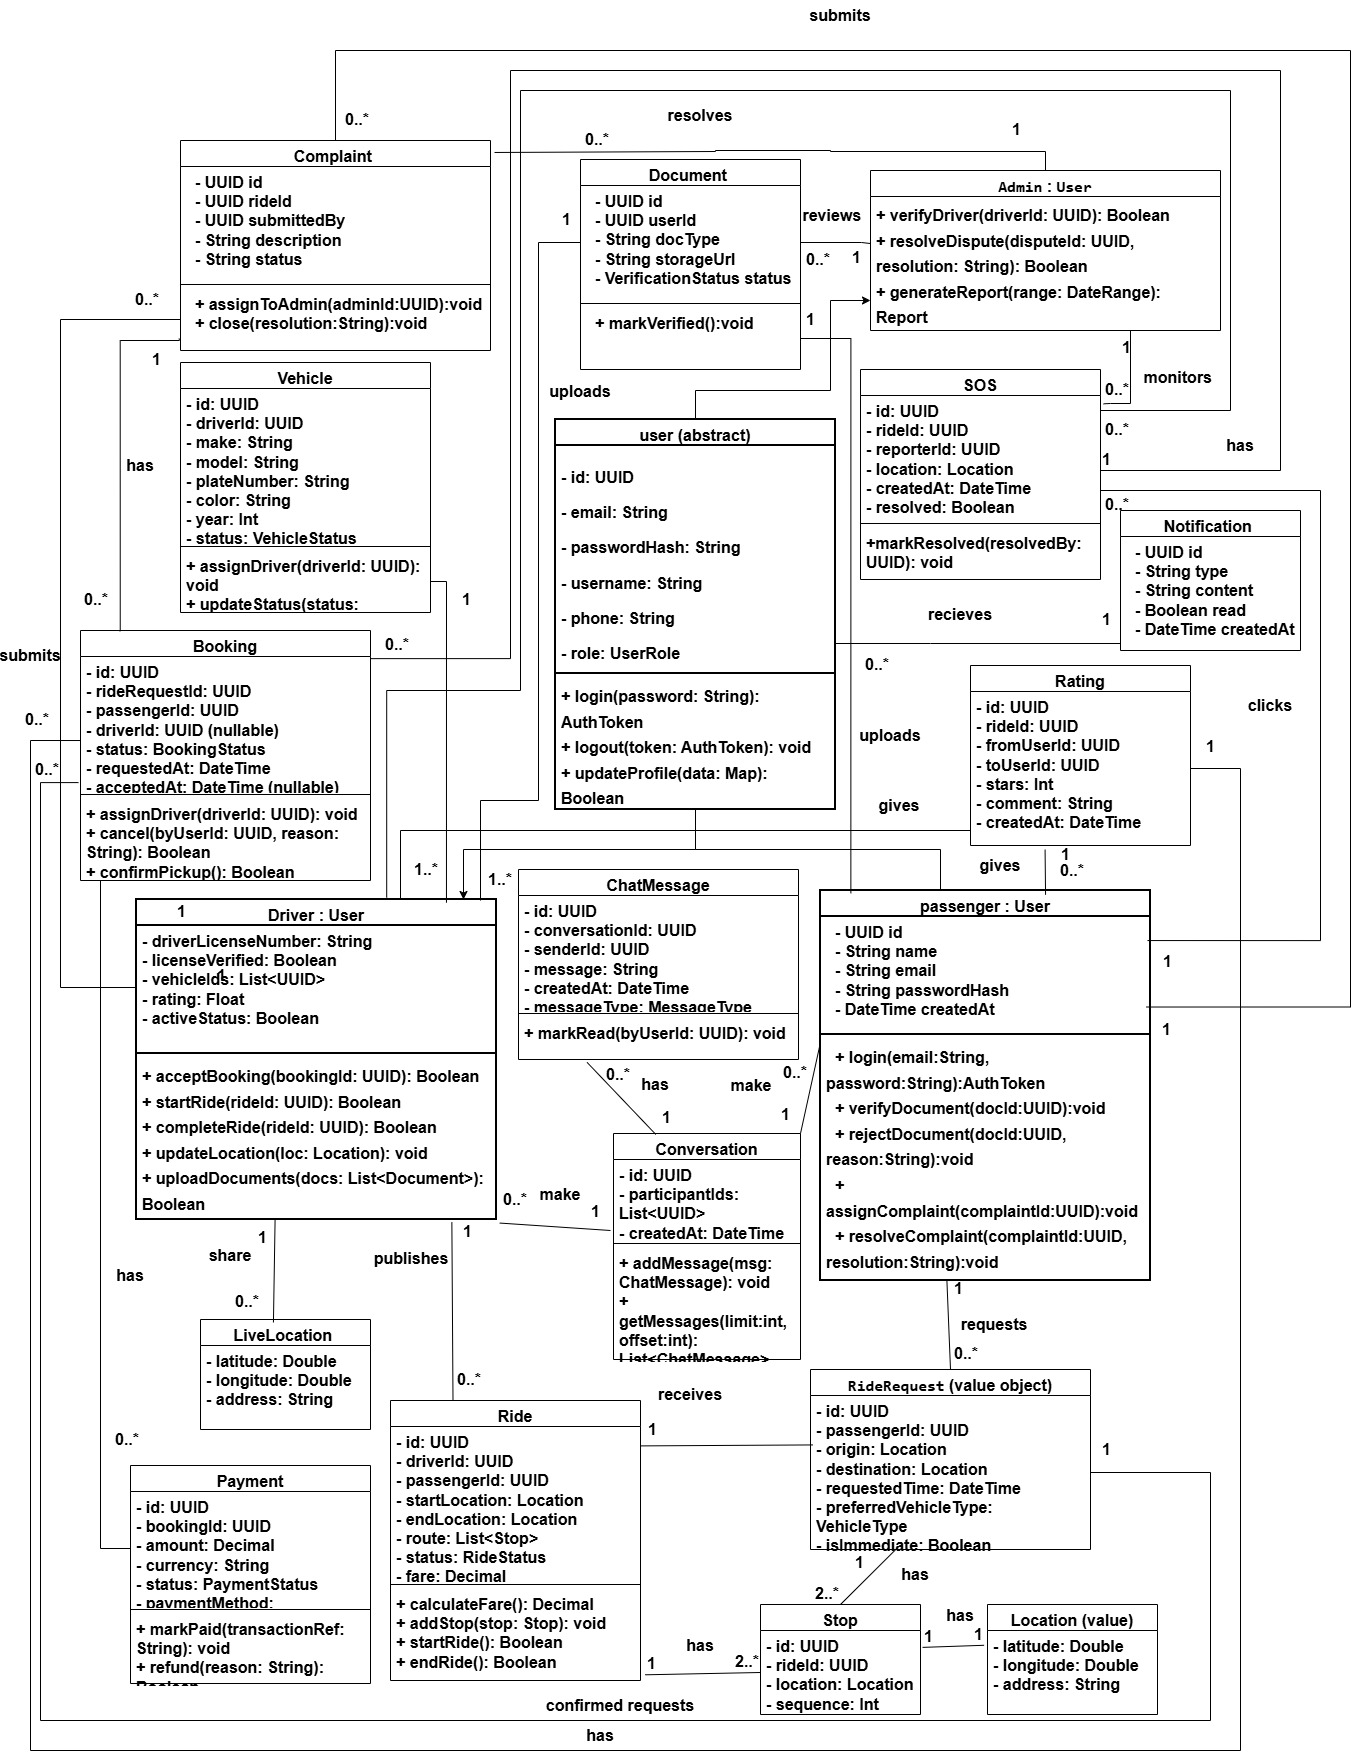
\includegraphics[width=0.9\textwidth,keepaspectratio,height=0.8\textheight]{assets/class diagram.jpg}
\caption{Comprehensive Class Diagram showing all system entities and relationships}
\label{fig:class}
\end{figure}

\subsubsection{Key Classes and Responsibilities}

\begin{itemize}
    \item \textbf{User (Abstract):} Base class with attributes: user\_id, name, email, password\_hash, role, created\_at. Methods: login(), logout(), updateProfile().
    
    \item \textbf{Passenger (inherits User):} Additional attributes: preference\_data (JSON). Methods: searchRides(), bookRide(), rateDriver(), fileComplaint().
    
    \item \textbf{Driver (inherits User):} Additional attributes: license\_number, verification\_status. Methods: createRide(), acceptBooking(), startRide(), completeRide().
    
    \item \textbf{Vehicle:} Attributes: vehicle\_id, driver\_id (FK), model, plate\_number, color, capacity, images. Methods: addVehicle(), updateVehicle(), deleteVehicle().
    
    \item \textbf{Ride:} Attributes: ride\_id, driver\_id (FK), route\_polyline, stops, departure\_time, available\_seats, gender\_preference, fare, status. Methods: createRide(), updateRide(), cancelRide().
    
    \item \textbf{Booking:} Attributes: booking\_id, ride\_id (FK), passenger\_id (FK), pickup\_stop, drop\_stop, seats\_booked, total\_fare, status, special\_requests. Methods: requestBooking(), acceptBooking(), rejectBooking(), cancelBooking().
    
    \item \textbf{Payment:} Attributes: payment\_id, booking\_id (FK), amount, method (cash/bank), status, timestamp. Methods: markPaid(), confirmReceived().
    
    \item \textbf{ChatMessage:} Attributes: message\_id, ride\_id (FK), sender\_id (FK), message\_text, timestamp, is\_broadcast. Methods: sendMessage(), getMessages().
    
    \item \textbf{Complaint:} Attributes: complaint\_id, ride\_id (FK), submitted\_by (FK), description, evidence\_links, status. Methods: fileComplaint(), resolveComplaint().
    
    \item \textbf{SOSRequest:} Attributes: sos\_id, user\_id (FK), ride\_id (FK), location, timestamp, status. Methods: triggerSOS(), escalateSOS(), resolveSOS().
    
    \item \textbf{User Document Fields:} User profile records store document/image URLs (CNIC, license, vehicle, profile photo) that reference uploaded files persisted in Supabase Storage. These fields support admin-driven verification workflows.
\end{itemize}

\subsubsection{Relationships}

\begin{itemize}
    \item \textbf{Inheritance:} Passenger and Driver inherit from User
    \item \textbf{One-to-Many:} Driver $\rightarrow$ Vehicle, Driver $\rightarrow$ Ride, Passenger $\rightarrow$ Booking, User $\rightarrow$ SOSRequest
    \item \textbf{Many-to-One:} Booking $\rightarrow$ Ride, Booking $\rightarrow$ Passenger, Ride $\rightarrow$ Driver
    \item \textbf{One-to-One:} Booking $\rightarrow$ Payment, Ride $\rightarrow$ Route (composition)
    \item \textbf{Many-to-Many:} Resolved through association classes like ChatMessage (connects Ride and User)
\end{itemize}

%===========================================================
\subsection{Sequence Diagrams}

Sequence diagrams show interaction between objects over time, illustrating request-response flows and component interactions.

\subsubsection{Sequence Diagram – Authentication (Login/Signup)}

\begin{figure}[H]
\centering
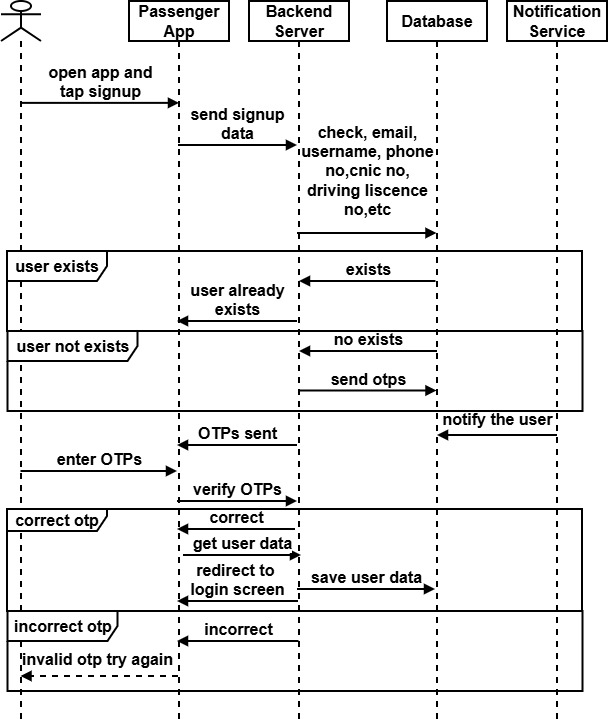
\includegraphics[width=0.8\textwidth,keepaspectratio,height=0.55\textheight]{assets/sequence diagrams/sequence diagram-USER SIGNUP (REGISTRATION).jpg}
\caption{Sequence Diagram - User Authentication (Signup and Login)}
\label{fig:seq_auth}
\end{figure}

\textbf{Description:} This diagram shows the interaction for user signup: User enters details, app sends to backend, backend validates, creates user record, sends OTP via Notification Service, user enters OTP, backend verifies and sets status to PENDING\_ADMIN\_VERIFICATION. For login: user enters credentials, backend validates, checks verification status, and returns JWT token.

\clearpage

\subsubsection{Sequence Diagram – Ride Posting}

\begin{figure}[H]
\centering
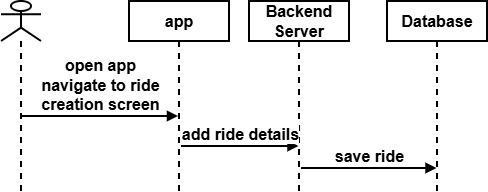
\includegraphics[width=1.0\textwidth,keepaspectratio,height=0.75\textheight]{assets/sequence diagrams/sequence diagram-post a ride.jpg}
\caption{Sequence Diagram - Driver Posting a Ride}
\label{fig:seq_ride_post}
\end{figure}

\textbf{Description:} Driver opens map, selects stops (interacting with Map Service for geocoding), enters ride parameters, backend validates, calculates fare (using FareCalculator), stores ride in database, and confirms creation. Ride becomes visible in marketplace.

\clearpage

\subsubsection{Sequence Diagram – Booking + Driver Acceptance}

\begin{figure}[H]
\centering
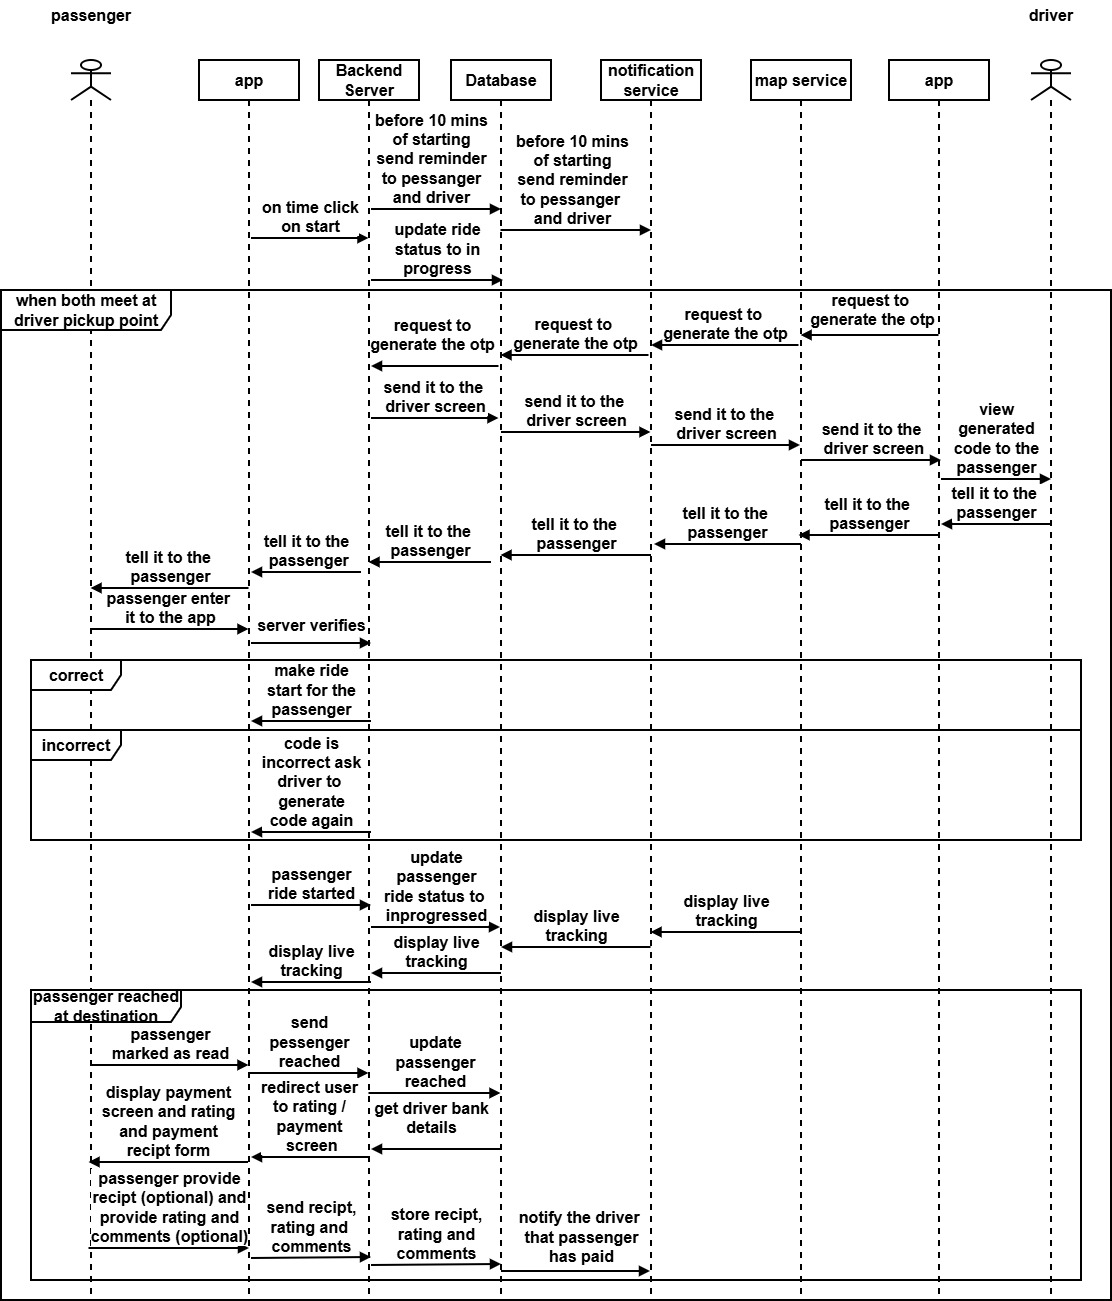
\includegraphics[width=0.9\textwidth,keepaspectratio,height=0.8\textheight]{assets/sequence diagrams/sequence diagram-post ride (starting to reached).jpg}
\caption{Sequence Diagram - Passenger Booking and Driver Acceptance}
\label{fig:seq_booking}
\end{figure}

\textbf{Description:} Passenger selects ride, selects stops/seats, backend calculates fare, locks seats, creates booking with REQUESTED status, sends notification to driver. Driver views request, accepts, backend updates booking to CONFIRMED, decrements available seats, sends confirmation to passenger.

\clearpage

\subsubsection{Sequence Diagram – Live Tracking + Ride Completion + Payment}

\begin{figure}[H]
\centering
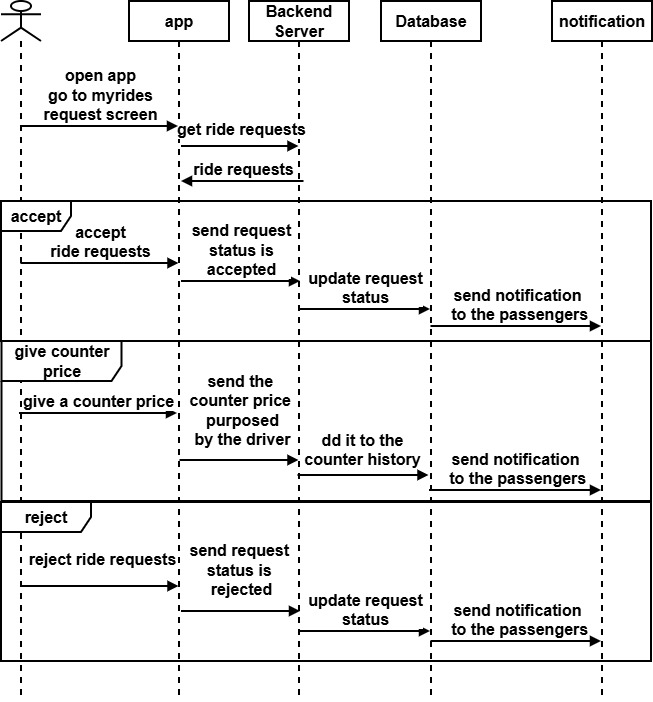
\includegraphics[width=0.9\textwidth,keepaspectratio,height=0.8\textheight]{assets/sequence diagrams/counter.jpg}
\caption{Sequence Diagram - Live Tracking, Ride Completion, and Payment}
\label{fig:seq_tracking}
\end{figure}

\textbf{Description:} Driver starts ride and sends periodic location updates to the backend via HTTP requests; passengers fetch updated tracking state through periodic HTTP updates. At destination, passenger marks reached, views driver bank details/QR, pays externally, marks paid. Driver confirms receipt, backend updates ride to COMPLETED, prompts ratings.

\clearpage

%===========================================================
\subsection{State Transition Diagrams}

State diagrams demonstrate how entities change state based on system events.

\subsubsection{State Transition Diagram – Ride Request and Booking}

\begin{figure}[H]
\centering
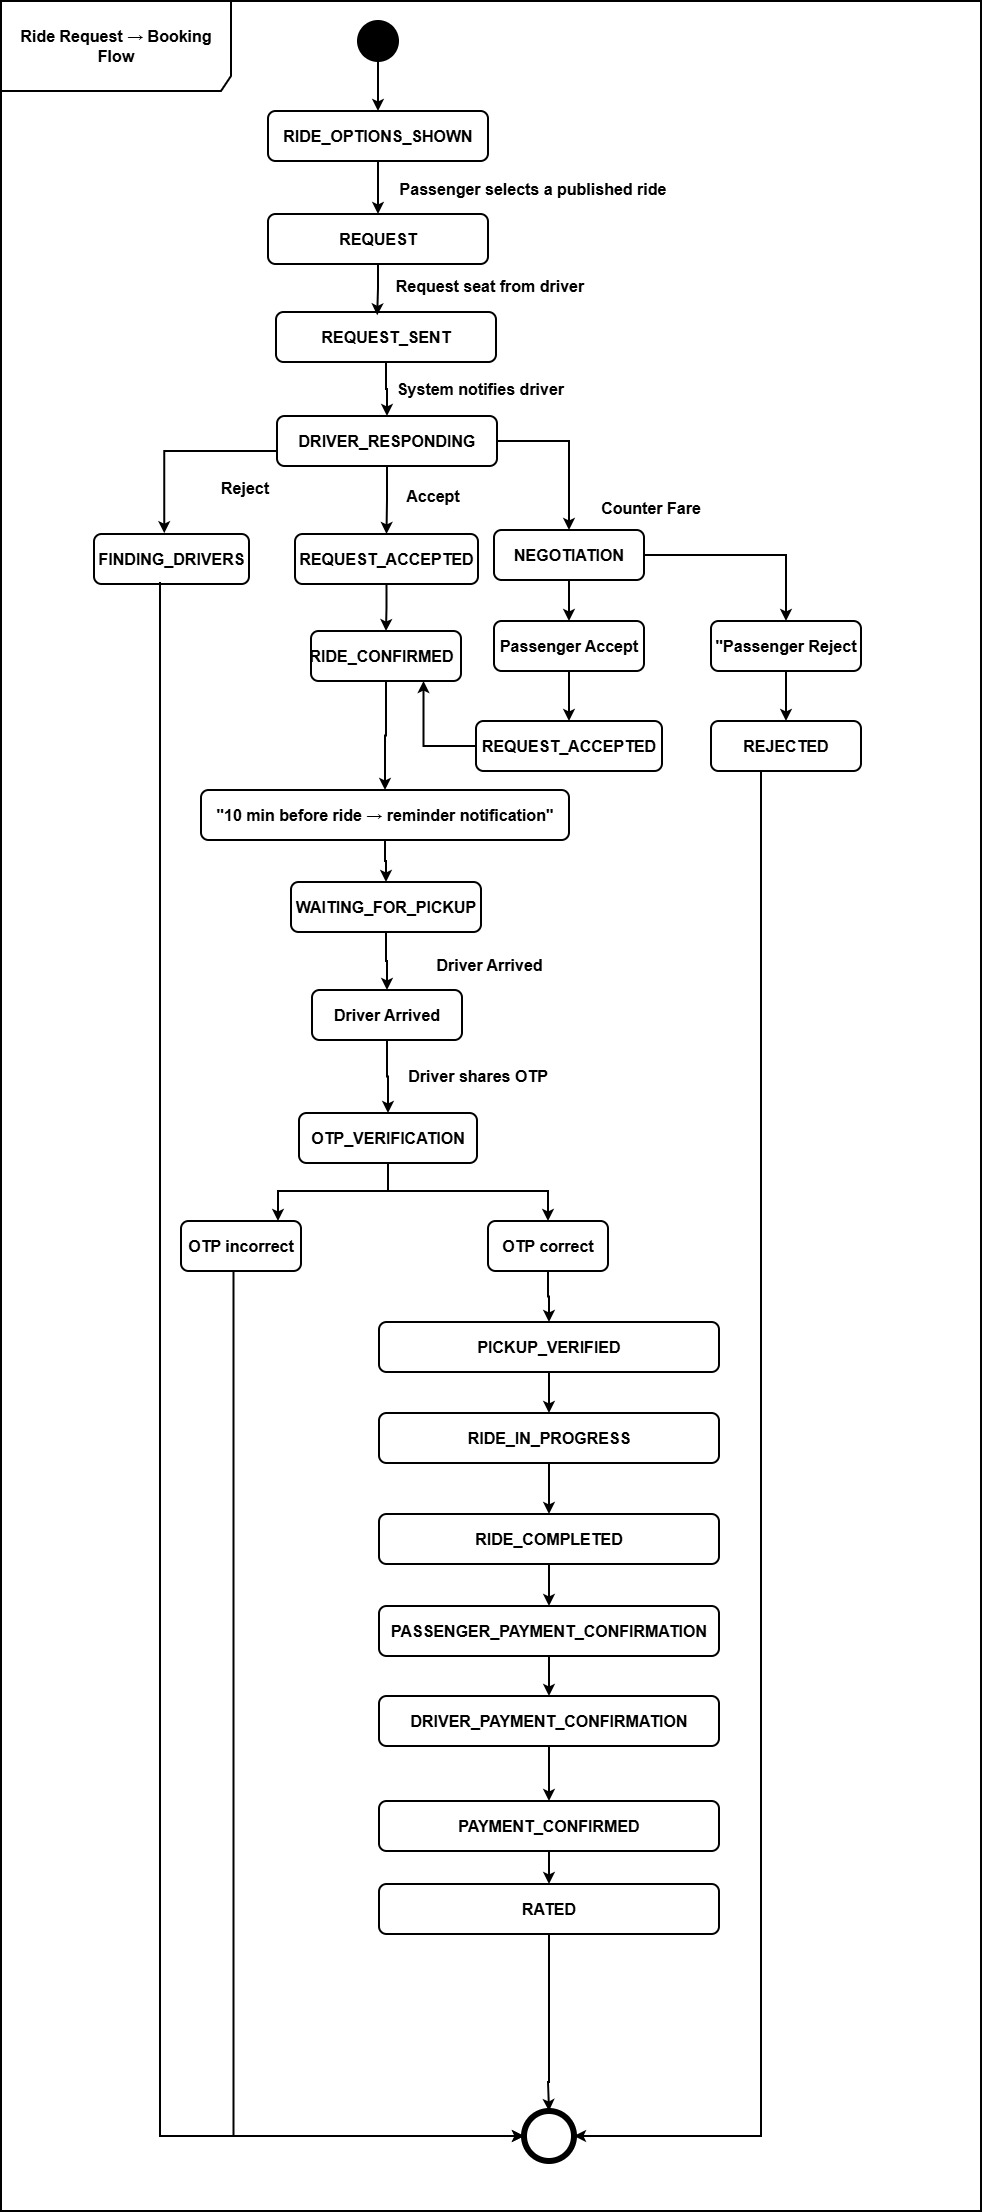
\includegraphics[width=0.9\textwidth,keepaspectratio,height=0.65\textheight]{assets/state transition diagrams/state transition-Ride Request → Booking Flow.jpg}
\caption{State Transition Diagram - Booking States}
\label{fig:state_booking}
\vspace{10pt}
\raggedright
\textbf{States:} 
\begin{itemize}[noitemsep,topsep=0pt]
    \item REQUESTED $\rightarrow$ (ACCEPTED $|$ REJECTED $|$ EXPIRED $|$ CANCELLED) $\rightarrow$ IN\_PROGRESS $\rightarrow$ COMPLETED
\end{itemize}
\textbf{Transitions:}
\begin{itemize}[noitemsep,topsep=0pt]
    \item Driver accepts (ACCEPTED), Driver rejects (REJECTED), Timeout (EXPIRED), Passenger cancels (CANCELLED), Ride starts (IN\_PROGRESS), Ride ends (COMPLETED)
\end{itemize}
\end{figure}

\subsubsection{State Transition Diagram – Driver States}

\begin{figure}[H]
\centering
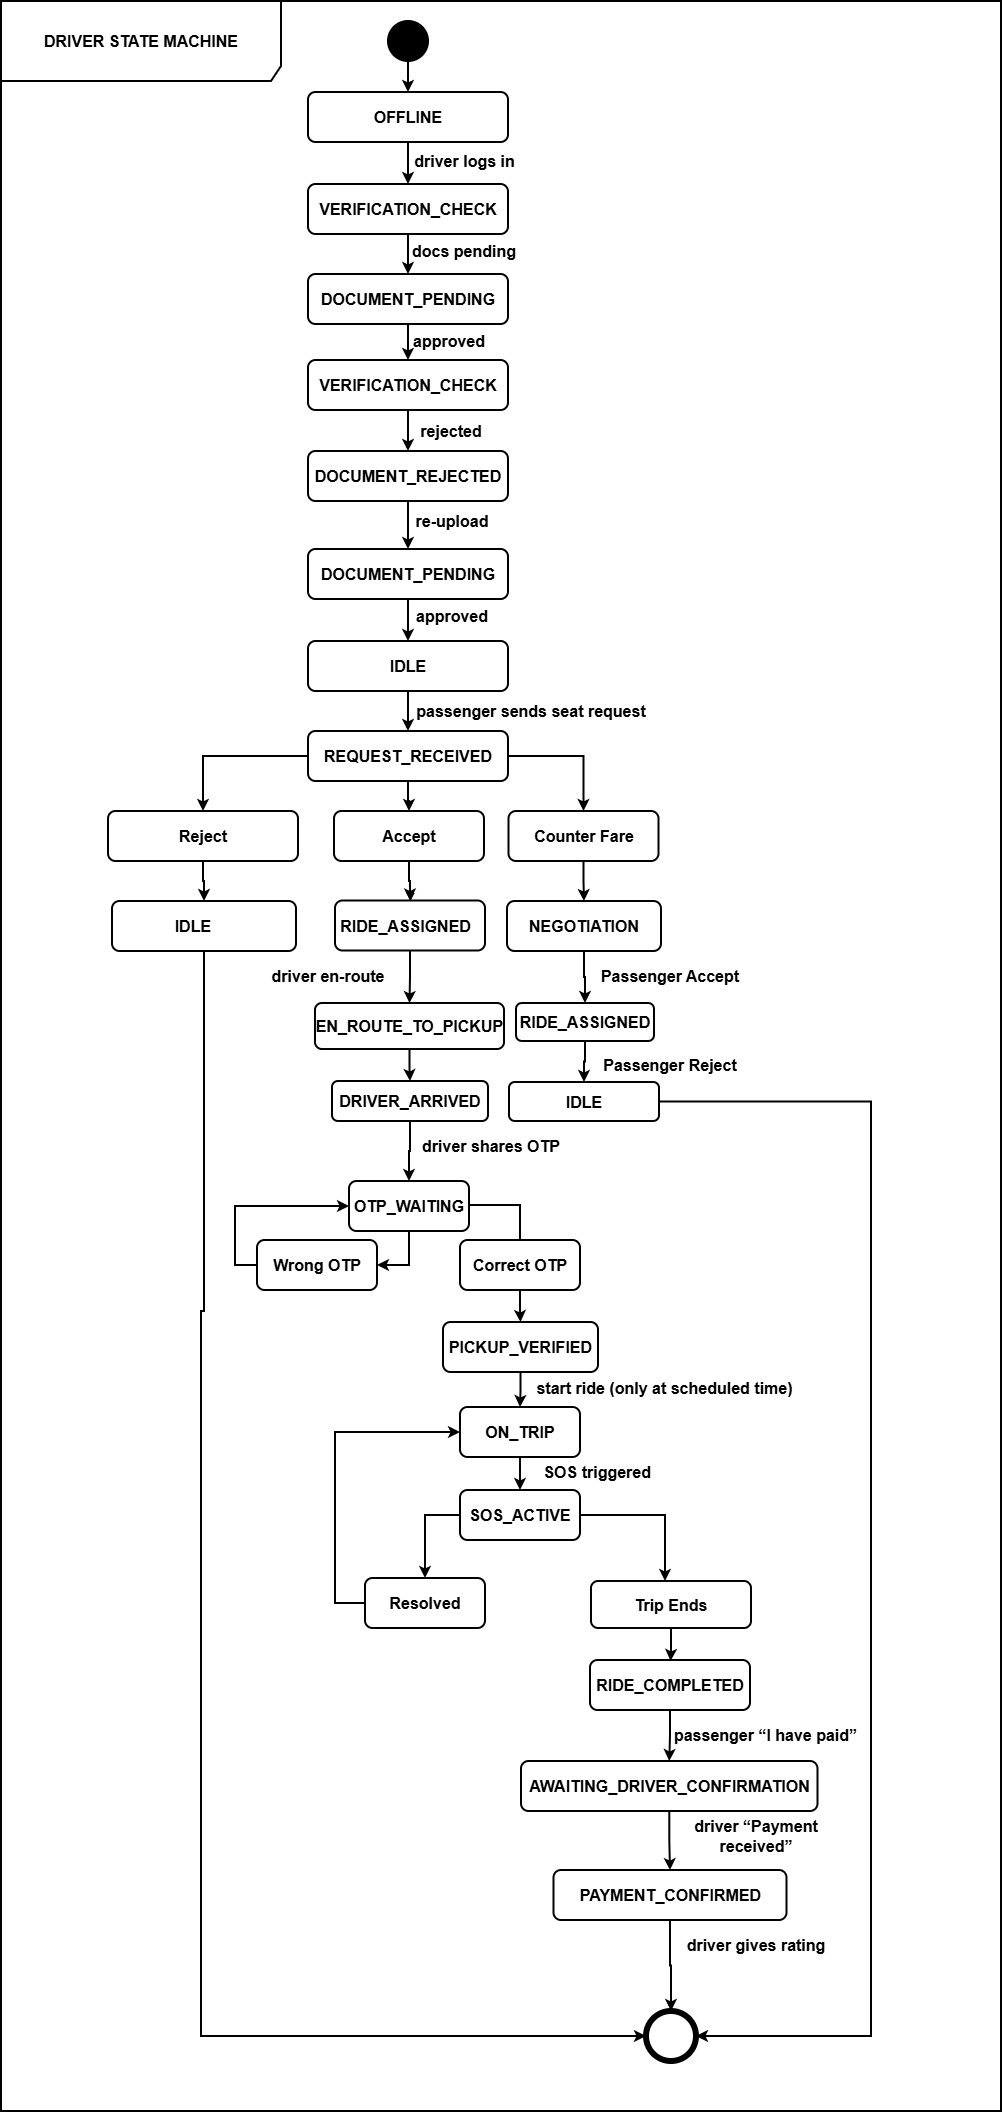
\includegraphics[width=0.9\textwidth,keepaspectratio,height=0.65\textheight]{assets/state transition diagrams/state transition-DRIVER STATE MACHINE.jpg}
\caption{State Transition Diagram - Driver States}
\label{fig:state_driver}
\vspace{10pt}
\raggedright
\textbf{States:} 
\begin{itemize}[noitemsep,topsep=0pt]
    \item OFFLINE $\rightarrow$ ONLINE $\rightarrow$ SEARCHING $\rightarrow$ ASSIGNED $\rightarrow$ EN\_ROUTE $\rightarrow$ ON\_RIDE $\rightarrow$ COMPLETED $\rightarrow$ ONLINE
\end{itemize}
\textbf{Transitions:}
\begin{itemize}[noitemsep,topsep=0pt]
    \item Driver logs in (ONLINE), receives request (SEARCHING), accepts (ASSIGNED), heading to pickup (EN\_ROUTE), passenger onboard (ON\_RIDE), ride ends (COMPLETED), becomes available (ONLINE)
\end{itemize}
\end{figure}

\subsubsection{State Transition Diagram – Passenger States}

\begin{figure}[H]
\centering
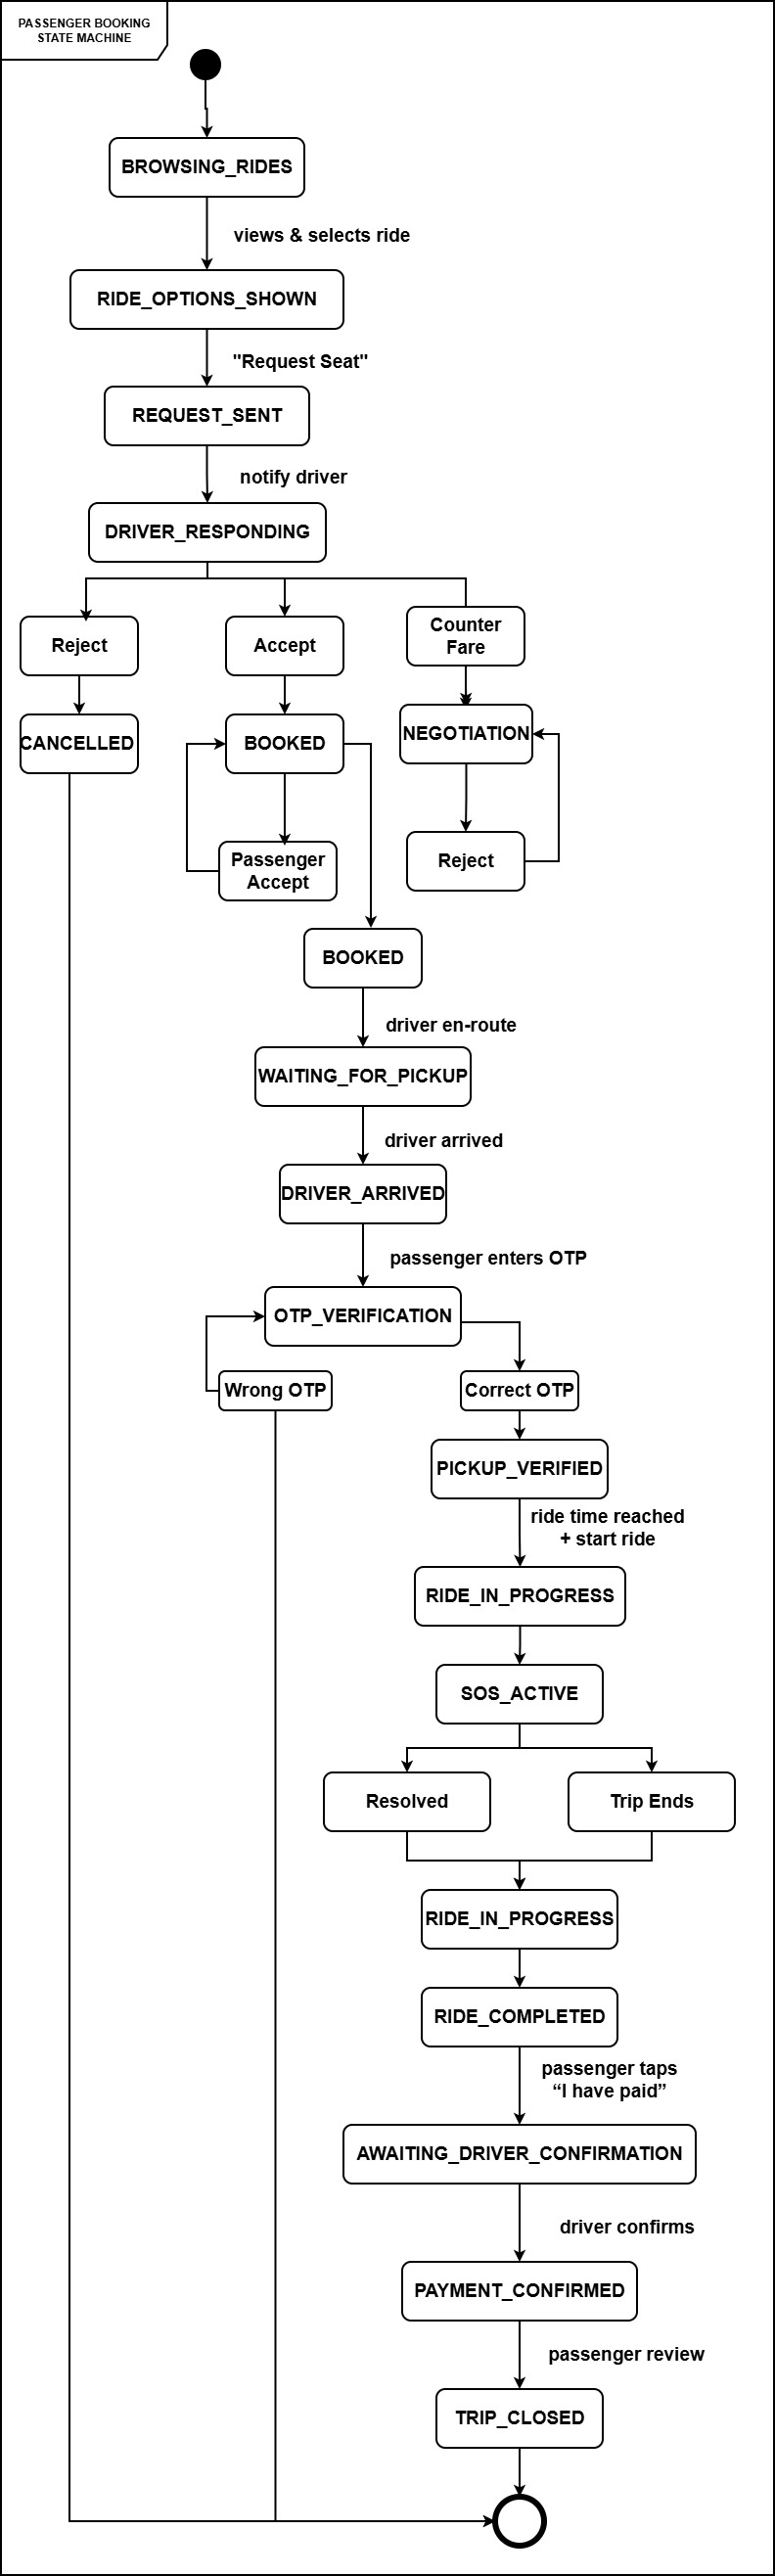
\includegraphics[width=0.9\textwidth,keepaspectratio,height=0.65\textheight]{assets/state transition diagrams/state transition-ASSENGER BOOKING STATE MACHINE.jpg}
\caption{State Transition Diagram - Passenger States}
\label{fig:state_passenger}
\vspace{10pt}
\raggedright
\textbf{States:} 
\begin{itemize}[noitemsep,topsep=0pt]
    \item IDLE $\rightarrow$ SEARCHING $\rightarrow$ BOOKED $\rightarrow$ WAITING $\rightarrow$ ON\_RIDE $\rightarrow$ COMPLETED $\rightarrow$ IDLE
\end{itemize}
\textbf{Transitions:}
\begin{itemize}[noitemsep,topsep=0pt]
    \item Searches rides (SEARCHING), books (BOOKED), driver accepted (WAITING), driver arrived/pickup (ON\_RIDE), dropped off (COMPLETED)
\end{itemize}
\end{figure}

\subsubsection{State Transition Diagram – SOS States}

\begin{figure}[H]
\centering
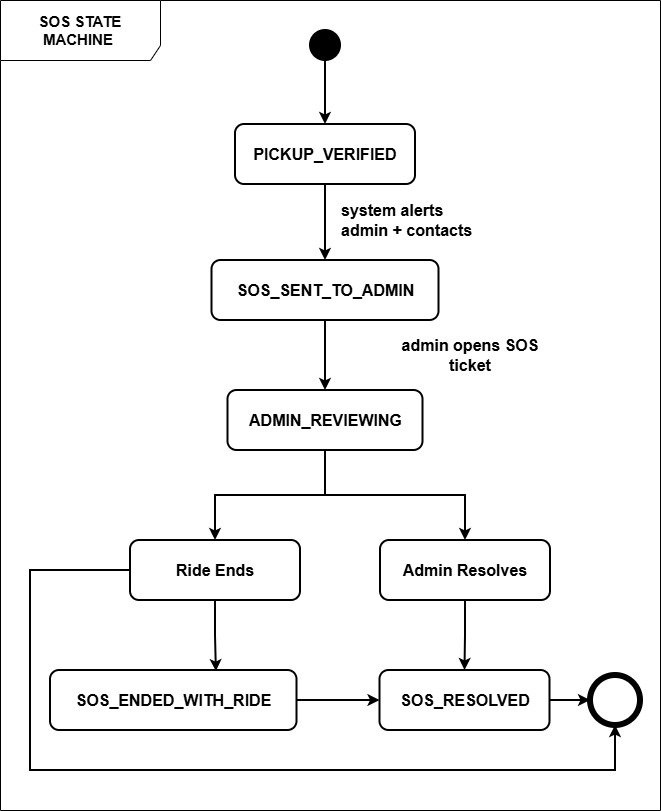
\includegraphics[width=0.9\textwidth,keepaspectratio,height=0.65\textheight]{assets/state transition diagrams/state transition-SOS STATE MACHINE — DRAW.IO READY.jpg}
\caption{State Transition Diagram - SOS States}
\label{fig:state_sos}
\vspace{10pt}
\raggedright
\textbf{States:} 
\begin{itemize}[noitemsep,topsep=0pt]
    \item INACTIVE $\rightarrow$ TRIGGERED $\rightarrow$ NOTIFIED $\rightarrow$ ACKNOWLEDGED $\rightarrow$ RESOLVED $\rightarrow$ INACTIVE
\end{itemize}
\textbf{Transitions:}
\begin{itemize}[noitemsep,topsep=0pt]
    \item User presses SOS (TRIGGERED), notifications sent (NOTIFIED), admin/contacts respond (ACKNOWLEDGED), situation resolved (RESOLVED)
\end{itemize}
\end{figure}

\subsubsection{Complaint and Dispute States Machine}

\begin{figure}[H]
\centering
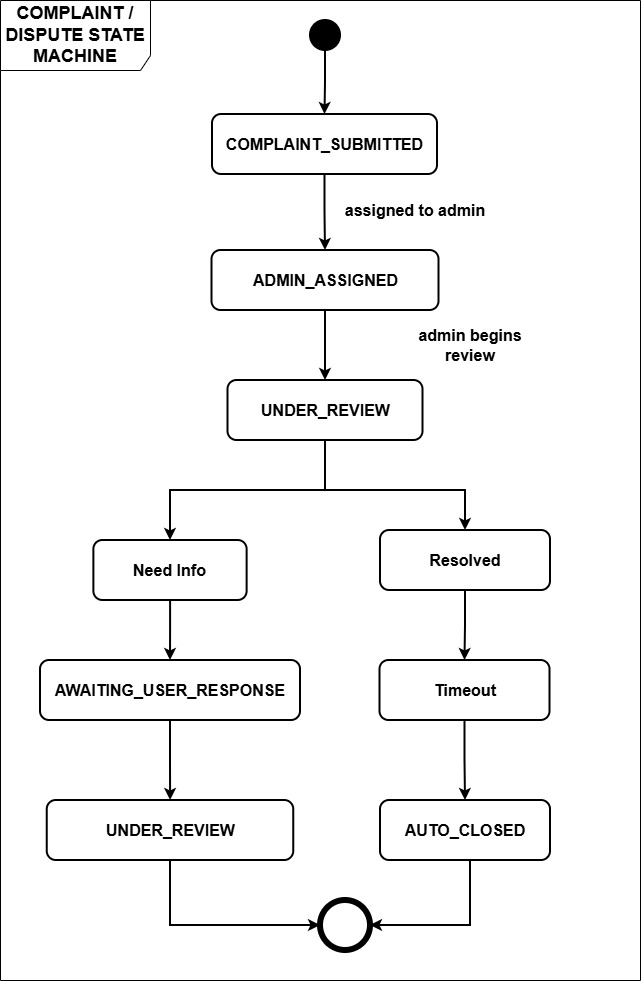
\includegraphics[width=0.9\textwidth,keepaspectratio,height=0.65\textheight]{assets/state transition diagrams/DISPUTE STATE MACHINE.jpg}
\caption{State Transition Diagram - Complaint and Dispute States}
\label{fig:state_dispute}
\vspace{10pt}
\raggedright
\textbf{States:} 
\begin{itemize}[noitemsep,topsep=0pt]
    \item FILED $\rightarrow$ UNDER\_REVIEW $\rightarrow$ (RESOLVED $|$ REJECTED $|$ ESCALATED)
\end{itemize}
\textbf{Transitions:}
\begin{itemize}[noitemsep,topsep=0pt]
    \item User files complaint (FILED), admin starts review (UNDER\_REVIEW), admin decides (RESOLVED/REJECTED), insufficient info (ESCALATED)
\end{itemize}
\end{figure}

\clearpage

\section{Data Flow Diagrams}
%===========================================================

Data Flow Diagrams (DFD) describe how data moves within the system at different levels of abstraction.

\subsection{Level 1 Data Flow Diagrams}

\subsubsection{Authentication \& Onboarding (Register, OTP, Admin verify)}

\begin{figure}[H]
\centering
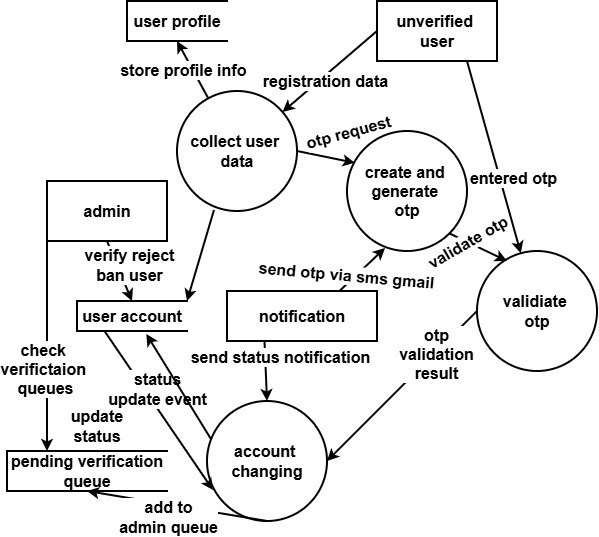
\includegraphics[width=0.9\textwidth,keepaspectratio,height=0.65\textheight]{assets/DFD/first registration module.jpg}
\caption{Level 1 DFD - Authentication and Onboarding}
\label{fig:dfd_auth}
\vspace{10pt}
\raggedright
\textbf{Processes:} 
\begin{itemize}[noitemsep,topsep=0pt]
    \item Register User, Send OTP, Verify OTP, Admin Verify Documents
\end{itemize}
\textbf{Data Stores:} 
\begin{itemize}[noitemsep,topsep=0pt]
    \item User DB, Document Store
\end{itemize}
\end{figure}

\subsubsection{Document Management (uploads \& verification)}

\begin{figure}[H]
\centering
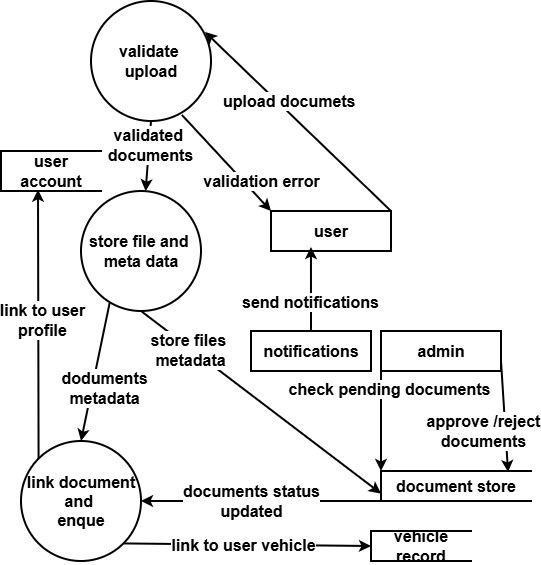
\includegraphics[width=0.9\textwidth,keepaspectratio,height=0.65\textheight]{assets/DFD/second module documents registartion.jpg}
\caption{Level 1 DFD - Document Management}
\label{fig:dfd_document}
\vspace{10pt}
\raggedright
\textbf{Processes:} 
\begin{itemize}[noitemsep,topsep=0pt]
    \item Upload Document, Validate Document, Store Document, Verify Document
\end{itemize}
\textbf{Data Stores:} 
\begin{itemize}[noitemsep,topsep=0pt]
    \item Document Store, User DB
\end{itemize}
\textbf{External Entities:} 
\begin{itemize}[noitemsep,topsep=0pt]
    \item User, Admin, Storage Service
\end{itemize}
\end{figure}


\subsubsection{Vehicle Management (add/edit/delete vehicles)}

\begin{figure}[H]
\centering
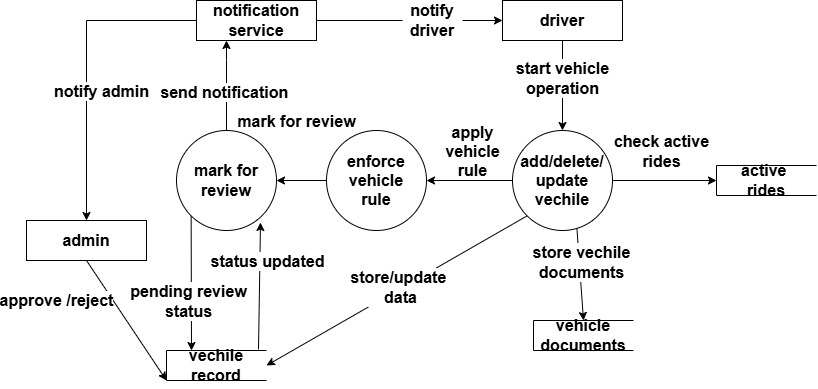
\includegraphics[width=0.9\textwidth,keepaspectratio,height=0.40\textheight]{assets/DFD/3rd module add vechile.jpg}
\caption{Level 1 DFD - Vehicle Management}
\label{fig:dfd_vehicle}
\vspace{10pt}
\raggedright
\textbf{Processes:} 
\begin{itemize}[noitemsep,topsep=0pt]
    \item Add Vehicle, Edit Vehicle, Delete Vehicle, Validate Vehicle
\end{itemize}
\textbf{Data Stores:} 
\begin{itemize}[noitemsep,topsep=0pt]
    \item Vehicle DB, User DB
\end{itemize}
\textbf{External Entities:} 
\begin{itemize}[noitemsep,topsep=0pt]
    \item Driver, Admin
\end{itemize}
\end{figure}


\subsubsection{Ride Management (create/edit/cancel, route \& stops)}

\begin{figure}[H]
\centering
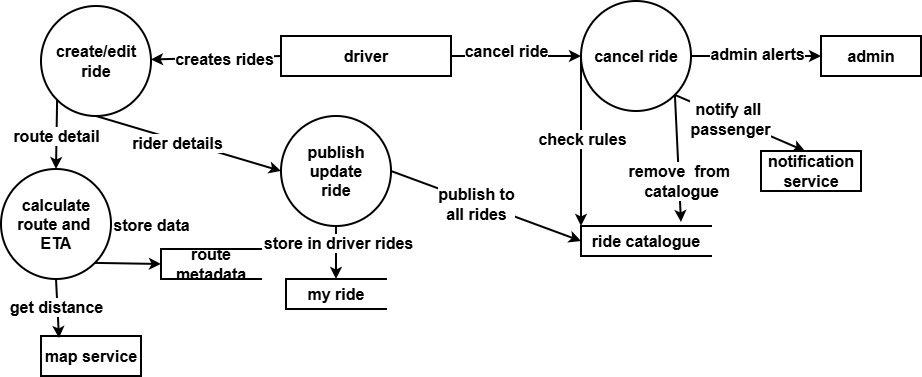
\includegraphics[width=0.9\textwidth,keepaspectratio,height=0.40\textheight]{assets/module_4_ride_management.jpg}
\caption{Level 1 DFD - Ride Management}
\label{fig:dfd_ride_mgmt}
\end{figure}

\clearpage

\raggedright
\textbf{Processes:} 
\begin{itemize}[noitemsep,topsep=0pt]
    \item Create Ride, Edit Ride, Cancel Ride, Calculate Fare
\end{itemize}
\textbf{Data Stores:} 
\begin{itemize}[noitemsep,topsep=0pt]
    \item Ride DB, Vehicle DB, Stop DB
\end{itemize}
\textbf{External Entities:} 
\begin{itemize}[noitemsep,topsep=0pt]
    \item Driver, Map Service
\end{itemize}

\subsubsection{Marketplace / Browse \& Search / Ride Details}

\begin{figure}[H]
\centering
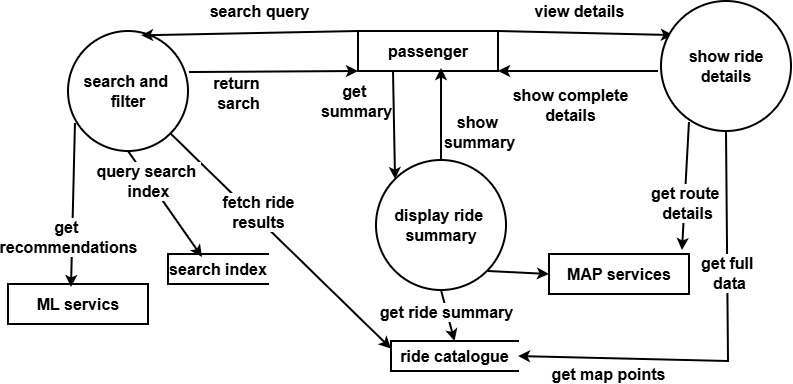
\includegraphics[width=0.9\textwidth,keepaspectratio,height=0.65\textheight]{assets/DFD/module 5 view rides.jpg}
\caption{Level 1 DFD - Ride Browsing and Search}
\label{fig:dfd_browse}
\vspace{10pt}
\raggedright
\textbf{Processes:} 
\begin{itemize}[noitemsep,topsep=0pt]
    \item Search Rides, Filter Rides, View Ride Details, Get Recommendations
\end{itemize}
\textbf{Data Stores:} 
\begin{itemize}[noitemsep,topsep=0pt]
    \item Ride DB, User DB
\end{itemize}
\textbf{External Entities:} 
\begin{itemize}[noitemsep,topsep=0pt]
    \item Passenger, ML Service
\end{itemize}
\end{figure}

\subsubsection{Booking \& Seat Management (select seats, lock seats)}

\begin{figure}[H]
\centering
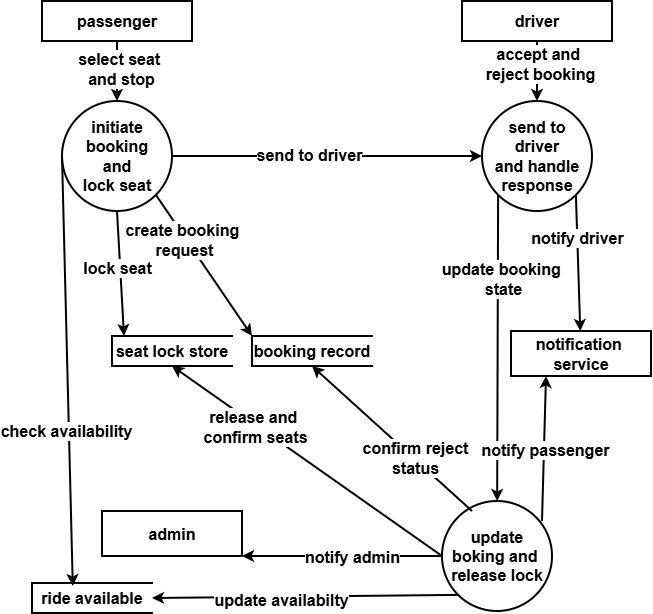
\includegraphics[width=0.9\textwidth,keepaspectratio,height=0.65\textheight]{assets/DFD/module 6 booking.jpg}
\caption{Level 1 DFD - Booking and Seat Management}
\label{fig:dfd_booking}
\vspace{10pt}
\raggedright
\textbf{Processes:} 
\begin{itemize}[noitemsep,topsep=0pt]
    \item Select Stops, Select Seats, Calculate Fare, Lock Seats, Create Booking
\end{itemize}
\textbf{Data Stores:} 
\begin{itemize}[noitemsep,topsep=0pt]
    \item Booking DB, Ride DB
\end{itemize}
\textbf{External Entities:} 
\begin{itemize}[noitemsep,topsep=0pt]
    \item Passenger, Driver
\end{itemize}
\end{figure}

\subsubsection{Post-Booking Chat / Messaging \& Broadcast}

\begin{figure}[H]
\centering
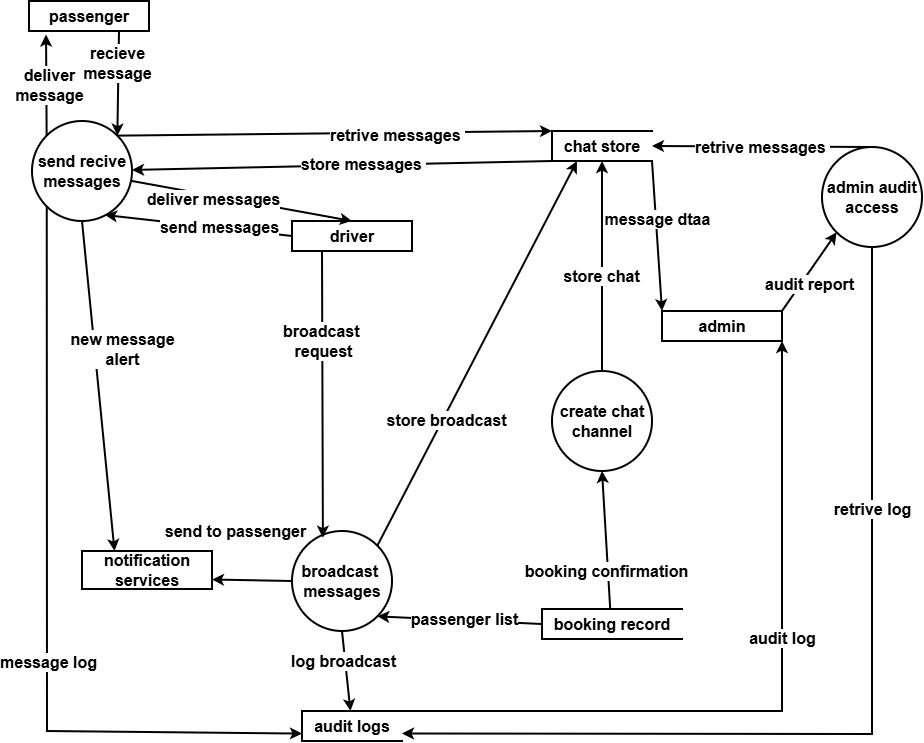
\includegraphics[width=0.9\textwidth,keepaspectratio,height=0.65\textheight]{assets/DFD/module 7 chat and message.jpg}
\caption{Level 1 DFD - Post-Booking Chat}
\label{fig:dfd_chat}
\vspace{10pt}
\raggedright
\textbf{Processes:} 
\begin{itemize}[noitemsep,topsep=0pt]
    \item Send Message, Broadcast Message, Store Message, Deliver Notification
\end{itemize}
\textbf{Data Stores:} 
\begin{itemize}[noitemsep,topsep=0pt]
    \item Chat DB
\end{itemize}
\textbf{External Entities:} 
\begin{itemize}[noitemsep,topsep=0pt]
    \item Passenger, Driver, Notification Service
\end{itemize}
\end{figure}


\subsubsection{Scheduler / Pre-Ride Reminders \& Permission Prompt}

\begin{figure}[H]
\centering
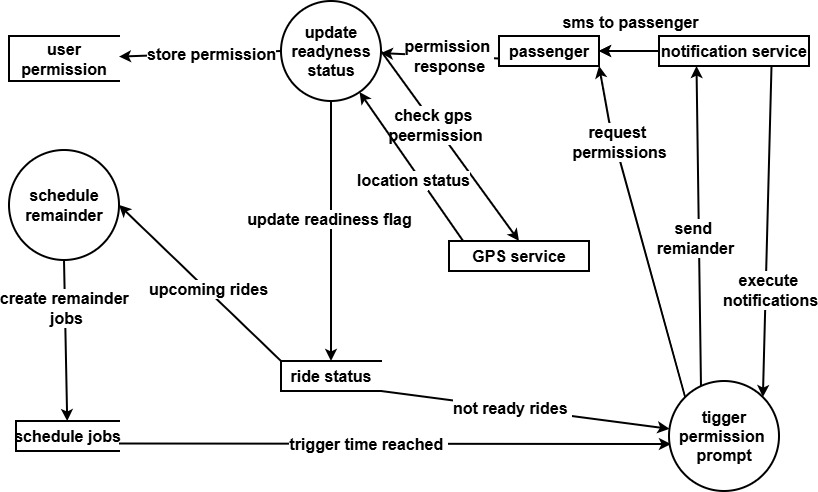
\includegraphics[width=0.9\textwidth,keepaspectratio,height=0.65\textheight]{assets/DFD/module 8 notification handlers.jpg}
\caption{Level 1 DFD - Pre-Ride Reminders}
\label{fig:dfd_reminder}
\vspace{10pt}
\raggedright
\textbf{Processes:} 
\begin{itemize}[noitemsep,topsep=0pt]
    \item Schedule Reminders, Send Reminders, Check Permissions, Update Readiness
\end{itemize}
\textbf{Data Stores:} 
\begin{itemize}[noitemsep,topsep=0pt]
    \item Ride DB, User DB
\end{itemize}
\textbf{External Entities:} 
\begin{itemize}[noitemsep,topsep=0pt]
    \item Passenger, Driver, Notification Service
\end{itemize}
\end{figure}

\subsubsection{Live Tracking \& Pickup Code (Start Ride / geofence)}

\begin{figure}[H]
\centering
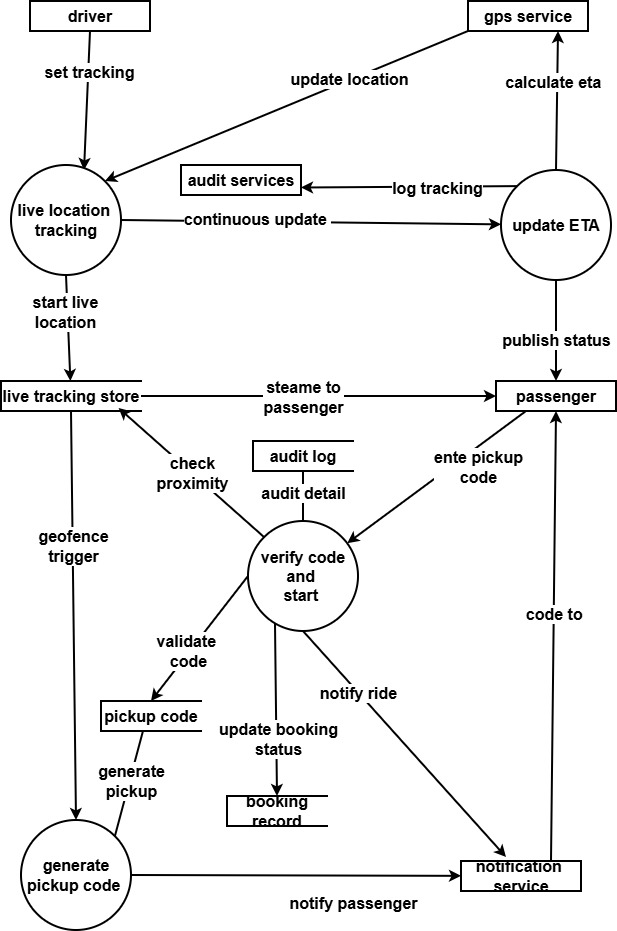
\includegraphics[width=0.9\textwidth,keepaspectratio,height=0.65\textheight]{assets/DFD/module 9 code verify.jpg}
\caption{Level 1 DFD - Live Tracking and Pickup Code}
\label{fig:dfd_tracking}
\vspace{10pt}
\raggedright
\textbf{Processes:} 
\begin{itemize}[noitemsep,topsep=0pt]
    \item Update Location, Broadcast Location, Generate Code, Verify Code, Start Ride
\end{itemize}
\textbf{Data Stores:} 
\begin{itemize}[noitemsep,topsep=0pt]
    \item Location DB, Ride DB
\end{itemize}
\textbf{External Entities:} 
\begin{itemize}[noitemsep,topsep=0pt]
    \item Driver, Passenger, Map Service
\end{itemize}
\end{figure}


\subsubsection{Payment \& Manual Payment Confirmation}

\begin{figure}[H]
\centering
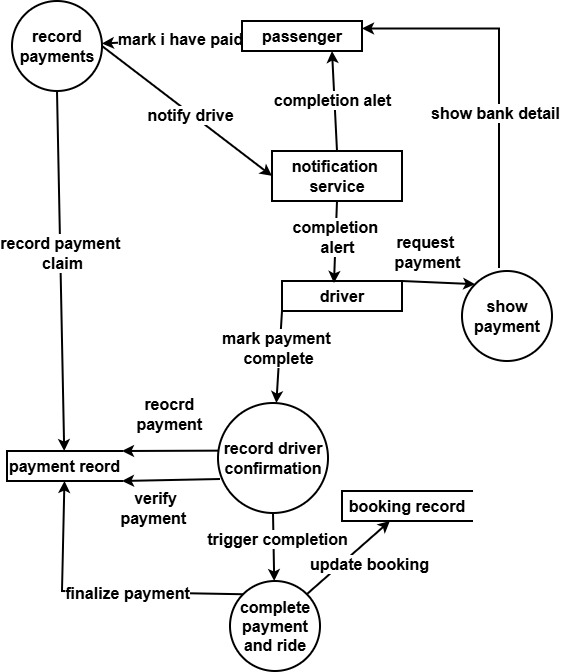
\includegraphics[width=0.9\textwidth,keepaspectratio,height=0.65\textheight]{assets/DFD/module 10 payment.jpg}
\caption{Level 1 DFD - Payment and Manual Confirmation}
\label{fig:dfd_payment}
\vspace{10pt}
\raggedright
\textbf{Processes:} 
\begin{itemize}[noitemsep,topsep=0pt]
    \item Show Payment Details, Mark Paid, Confirm Receipt, Update Ride Status
\end{itemize}
\textbf{Data Stores:} 
\begin{itemize}[noitemsep,topsep=0pt]
    \item Payment DB, Ride DB
\end{itemize}
\textbf{External Entities:} 
\begin{itemize}[noitemsep,topsep=0pt]
    \item Passenger, Driver, Notification Service
\end{itemize}
\end{figure}


\subsubsection{Ratings \& Completion Workflow}

\begin{figure}[H]
\centering
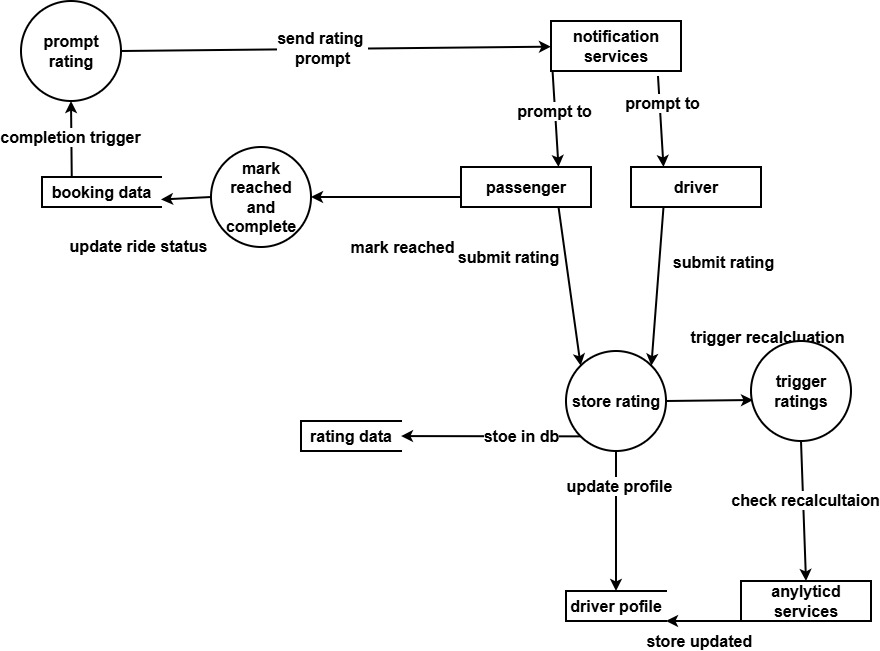
\includegraphics[width=0.9\textwidth,keepaspectratio,height=0.65\textheight]{assets/DFD/module 11 ratings.jpg}
\caption{Level 1 DFD - Ratings and Completion}
\label{fig:dfd_rating}
\vspace{10pt}
\raggedright
\textbf{Processes:} 
\begin{itemize}[noitemsep,topsep=0pt]
    \item Prompt Rating, Submit Rating, Update User Rating, Complete Ride
\end{itemize}
\textbf{Data Stores:} 
\begin{itemize}[noitemsep,topsep=0pt]
    \item Rating DB, Ride DB, User DB
\end{itemize}
\textbf{External Entities:} 
\begin{itemize}[noitemsep,topsep=0pt]
    \item Passenger, Driver
\end{itemize}
\end{figure}

\subsubsection{SOS / Emergency \& Incident Management}

\begin{figure}[H]
\centering
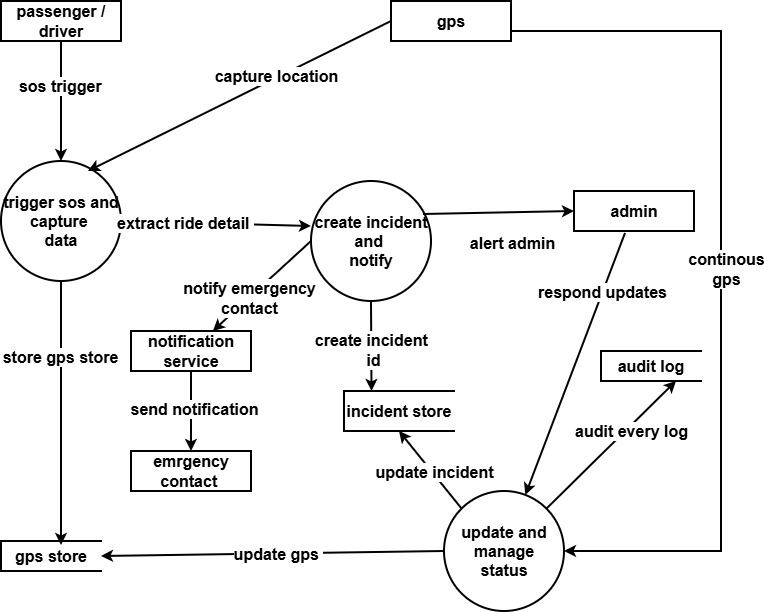
\includegraphics[width=0.9\textwidth,keepaspectratio,height=0.65\textheight]{assets/DFD/module 12.jpg}
\caption{Level 1 DFD - SOS and Emergency Management}
\label{fig:dfd_sos}
\vspace{10pt}
\raggedright
\textbf{Processes:} 
\begin{itemize}[noitemsep,topsep=0pt]
    \item Trigger SOS, Notify Contacts, Notify Admin, Log Incident, Escalate
\end{itemize}
\textbf{Data Stores:} 
\begin{itemize}[noitemsep,topsep=0pt]
    \item SOS DB, User DB, Ride DB
\end{itemize}
\textbf{External Entities:} 
\begin{itemize}[noitemsep,topsep=0pt]
    \item User, Emergency Contact, Admin, Notification Service
\end{itemize}
\end{figure}


\subsubsection{Dispute Management \& Admin Dashboard}

\begin{figure}[H]
\centering
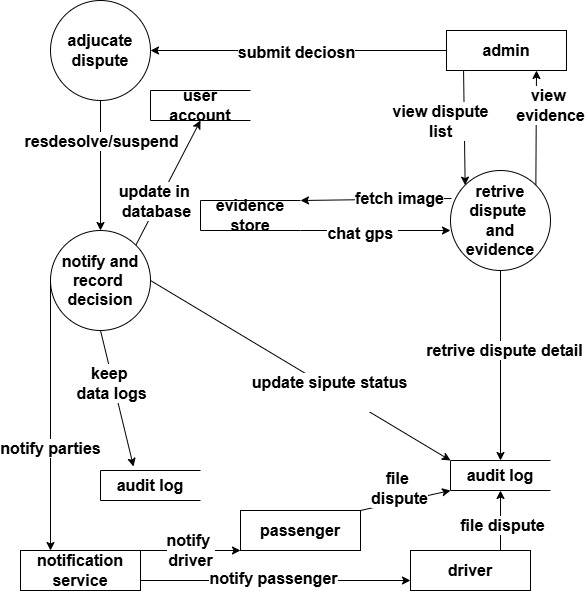
\includegraphics[width=0.9\textwidth,keepaspectratio,height=0.65\textheight]{assets/DFD/module13.jpg}
\caption{Level 1 DFD - Dispute Management}
\label{fig:dfd_dispute}
\vspace{10pt}
\raggedright
\textbf{Processes:} 
\begin{itemize}[noitemsep,topsep=0pt]
    \item File Dispute, View Dispute, Review Evidence, Resolve Dispute, Notify Parties
\end{itemize}
\textbf{Data Stores:} 
\begin{itemize}[noitemsep,topsep=0pt]
    \item Dispute DB, Chat DB, Location DB
\end{itemize}
\textbf{External Entities:} 
\begin{itemize}[noitemsep,topsep=0pt]
    \item User, Admin, Notification Service
\end{itemize}
\end{figure}


\subsubsection{Notification Service}

\begin{figure}[H]
\centering
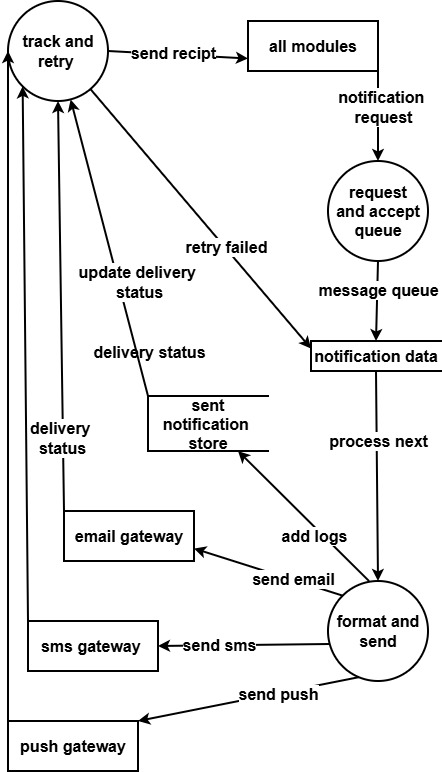
\includegraphics[width=0.9\textwidth,keepaspectratio,height=0.65\textheight]{assets/DFD/module14.jpg}
\caption{Level 1 DFD - Notification Service}
\label{fig:dfd_notification}
\vspace{10pt}
\raggedright
\textbf{Processes:} 
\begin{itemize}[noitemsep,topsep=0pt]
    \item Queue Notification, Send Push, Send SMS, Send Email, Log Delivery
\end{itemize}
\textbf{Data Stores:} 
\begin{itemize}[noitemsep,topsep=0pt]
    \item Notification Log DB
\end{itemize}
\textbf{External Entities:} 
\begin{itemize}[noitemsep,topsep=0pt]
    \item Application, FCM, SMS Gateway, Email Service
\end{itemize}
\end{figure}


\subsubsection{Recommendation (ML) Service}

\begin{figure}[H]
\centering
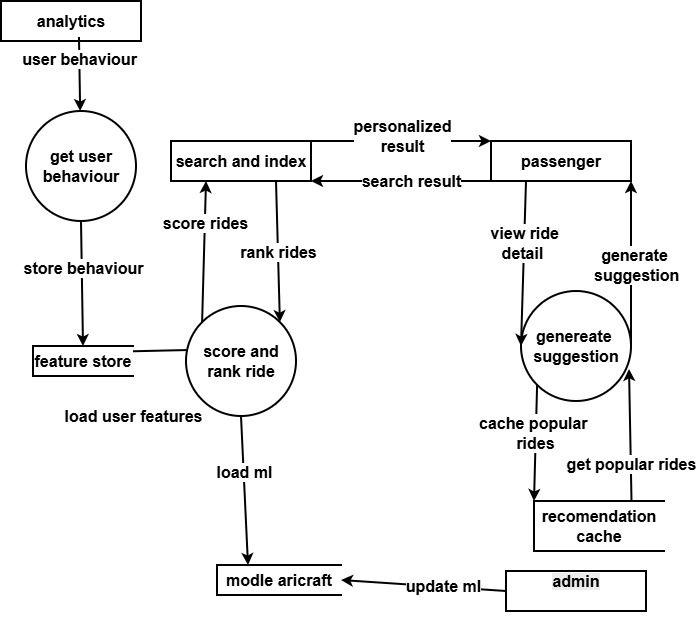
\includegraphics[width=0.9\textwidth,keepaspectratio,height=0.65\textheight]{assets/DFD/module15.jpg}
\caption{Level 1 DFD - ML Recommendation Service}
\label{fig:dfd_ml}
\vspace{10pt}
\raggedright
\textbf{Processes:} 
\begin{itemize}[noitemsep,topsep=0pt]
    \item Fetch User History, Build Feature Vectors, Compute Similarity, Rank Rides
\end{itemize}
\textbf{Data Stores:} 
\begin{itemize}[noitemsep,topsep=0pt]
    \item Ride DB, User History DB
\end{itemize}
\textbf{External Entities:} 
\begin{itemize}[noitemsep,topsep=0pt]
    \item Application, ML Model
\end{itemize}
\end{figure}


\subsubsection{Smart Chatbot Support}

\begin{figure}[H]
\centering
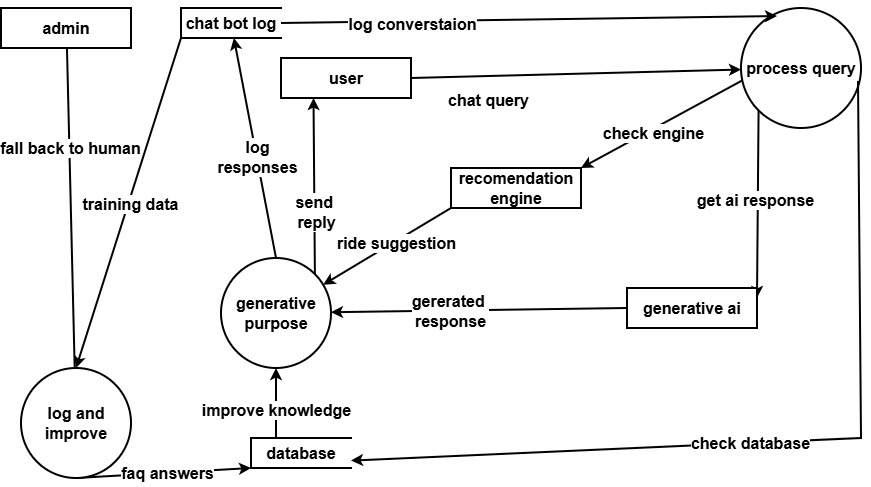
\includegraphics[width=0.9\textwidth,keepaspectratio,height=0.65\textheight]{assets/DFD/module16.jpg}
\caption{Level 1 DFD - Smart Chatbot Support}
\label{fig:dfd_chatbot}
\vspace{10pt}
\raggedright
\textbf{Processes:} 
\begin{itemize}[noitemsep,topsep=0pt]
    \item Parse Query, Classify Intent, Fetch FAQ, Call ML for Recommendations, Format Response
\end{itemize}
\textbf{Data Stores:} 
\begin{itemize}[noitemsep,topsep=0pt]
    \item FAQ KB, Ride DB
\end{itemize}
\textbf{External Entities:} 
\begin{itemize}[noitemsep,topsep=0pt]
    \item User, LLM API, ML Service
\end{itemize}
\end{figure}


\subsubsection{Audit / Logging / Analytics}

\begin{figure}[H]
\centering
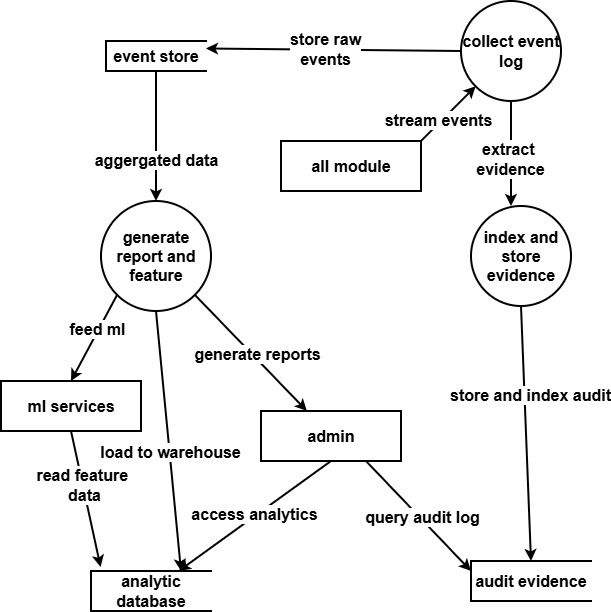
\includegraphics[width=0.9\textwidth,keepaspectratio,height=0.65\textheight]{assets/DFD/module17.jpg}
\caption{Level 1 DFD - Audit, Logging, and Analytics}
\label{fig:dfd_audit}
\vspace{10pt}
\raggedright
\textbf{Processes:} 
\begin{itemize}[noitemsep,topsep=0pt]
    \item Log Event, Store Log, Analyze Patterns, Generate Reports, Detect Fraud
\end{itemize}
\textbf{Data Stores:} 
\begin{itemize}[noitemsep,topsep=0pt]
    \item Audit Log DB
\end{itemize}
\textbf{External Entities:} 
\begin{itemize}[noitemsep,topsep=0pt]
    \item All System Components, Admin
\end{itemize}
\end{figure}

%===========================================================
\section{Data Design}
%===========================================================

This section describes how data is structured, stored, and managed.

\textbf{Guidelines:}
\begin{itemize}
    \item Define database type (SQL / NoSQL).
    \item Explain schema structure.
    \item Describe indexing strategy.
    \item Mention security mechanisms.
    \item Discuss scalability considerations.
\end{itemize}

The Data Design section explains the conversion of the information domain of the Lets Go Ride Sharing App - Ride Sharing and Recommendation System into logical and physical data structures. This contains data entities, relationships, storage plans as well as the entire schema of the database. 

It employs PostgreSQL as the relational database because it is stable, supports indexing, geospatial extensions and highly supports multiple simultaneous transactions, which is required in a ride-sharing system where drivers and riders interact in real-time. 

The data design will have the backend system and the external services dealing with accurate, normalized, and well-structured data.

\subsection{Entity Relationship Diagram (ERD)}

The Entity Relationship Diagram (ERD) represents the logical database structure of the system.

\textbf{Guidelines:}
\begin{itemize}
    \item Clearly identify all entities (tables/collections).
    \item Highlight Primary Keys (PK).
    \item Highlight Foreign Keys (FK).
    \item Show relationship cardinality (1:1, 1:N, M:N).
    \item Maintain consistency with database tables defined earlier.
\end{itemize}

\textbf{Include in ERD:}
\begin{itemize}
    \item \textbf{User Entity}: User (abstract superclass), Passenger, Driver.
    \item \textbf{Core Functional Entities}: RideRequest, Ride, Booking, Location.
    \item \textbf{Transaction/Log Entity}: Payment, Complaint, SOSRequest, ChatMessage.
    \item \textbf{Administrative Entity}: User verification state and user document/image URL fields.
\end{itemize}

\begin{sidewaysfigure}
\centering
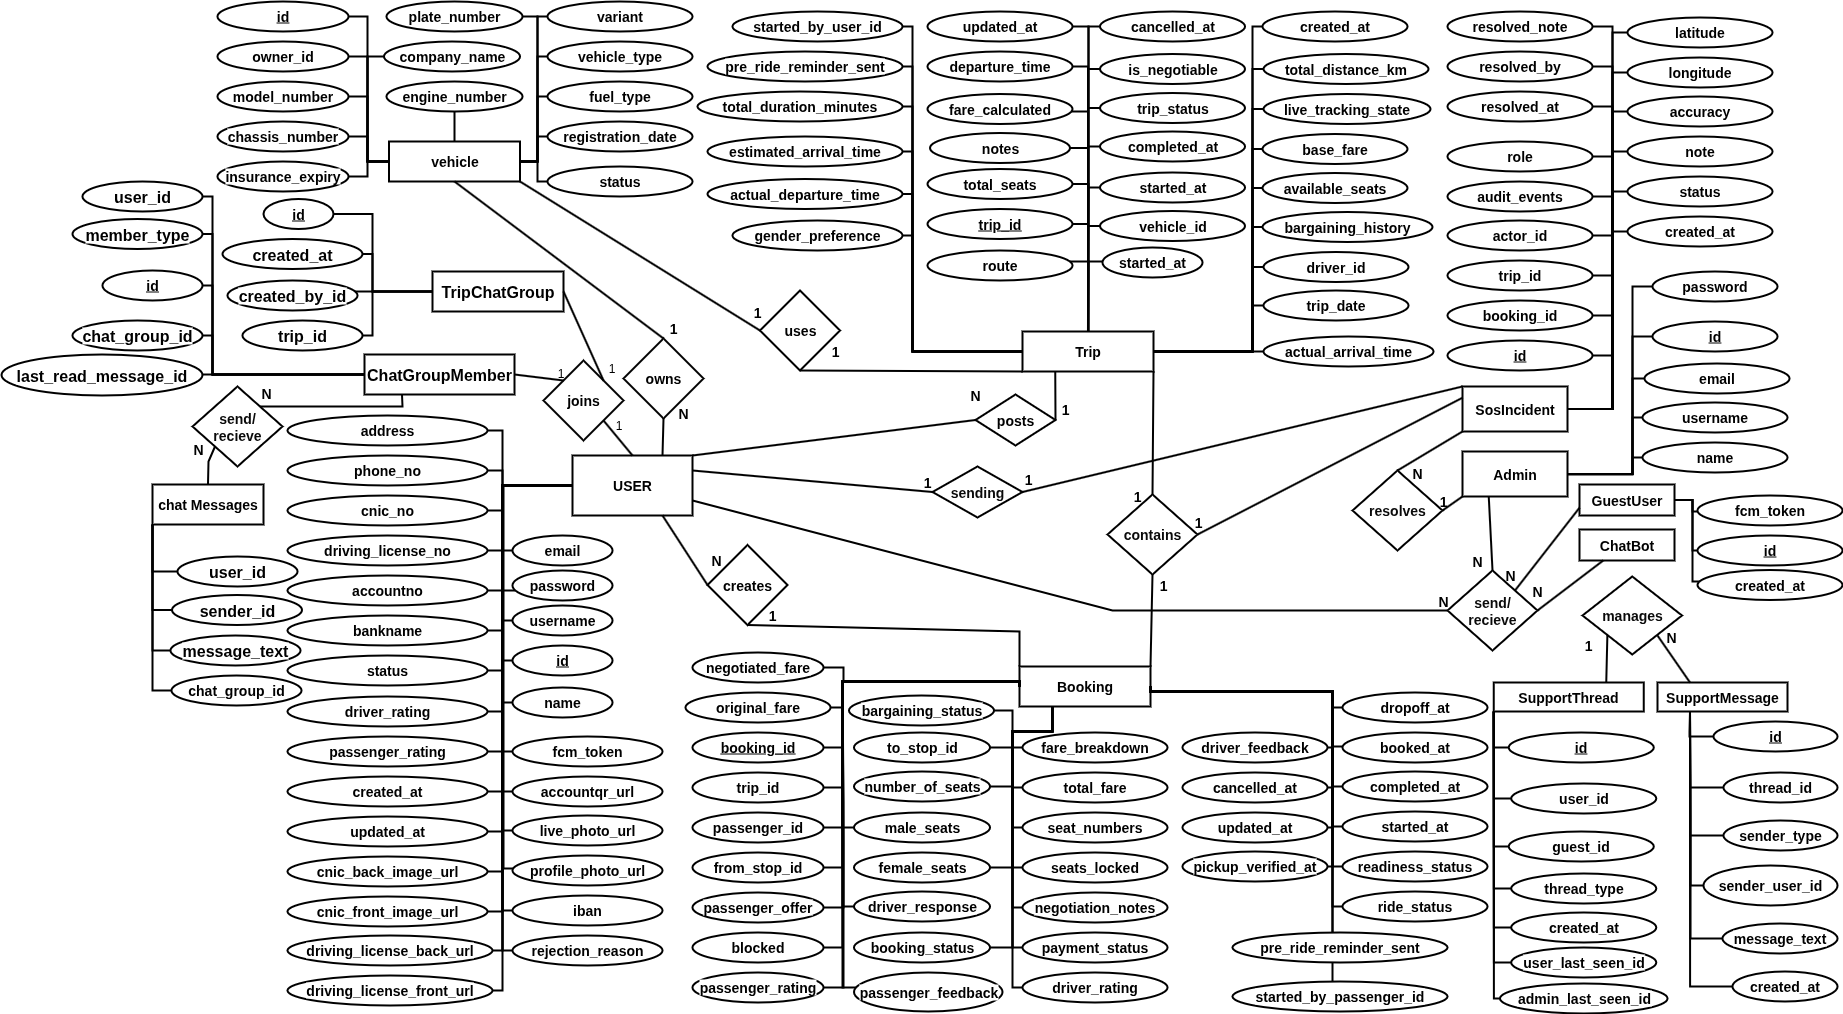
\includegraphics[width=1.0\linewidth,keepaspectratio]{assets/db_diagrams/ERD_DIAGRAMAS.png}
\caption{Entity Relationship Diagram}
\label{fig:erd_diagram}
\end{sidewaysfigure}

\subsection{Database Architecture}

\textbf{Explain:}
\begin{itemize}
    \item \textbf{Client-Server Architecture}: The data in the system are efficiently, safely, and scalably handled through a centralized relational approach.
    \item \textbf{Relational Storage (PostgreSQL)}: Used for User profiles, Rides, bookings, payments, SOS and complaints, Chat messages, and Documents metadata.
    \item \textbf{Geospatial Computation}: Distance calculations and route summaries are handled in application logic using geographic coordinates.
    \item \textbf{Cloud Storage}: Handled via Storage Service for Driver license images, CNIC images, and Profile pictures.
    \item \textbf{Caching Layer}: Optional caching can be applied for frequently accessed read-heavy data when needed.
\end{itemize}

%===========================================================
\section{Database Schema Diagram}
%===========================================================

The physical data model specifies actual database tables, columns, data types, primary keys, foreign keys, and constraints.

The Database Schema Diagram represents the physical database implementation structure.

\textbf{Guidelines:}
\begin{itemize}
    \item Show actual table structure.
    \item Include column names and data types.
    \item Show PK and FK relationships.
    \item Reflect normalization level (1NF, 2NF, 3NF if applicable).
\end{itemize}

\begin{figure}[H]
\centering
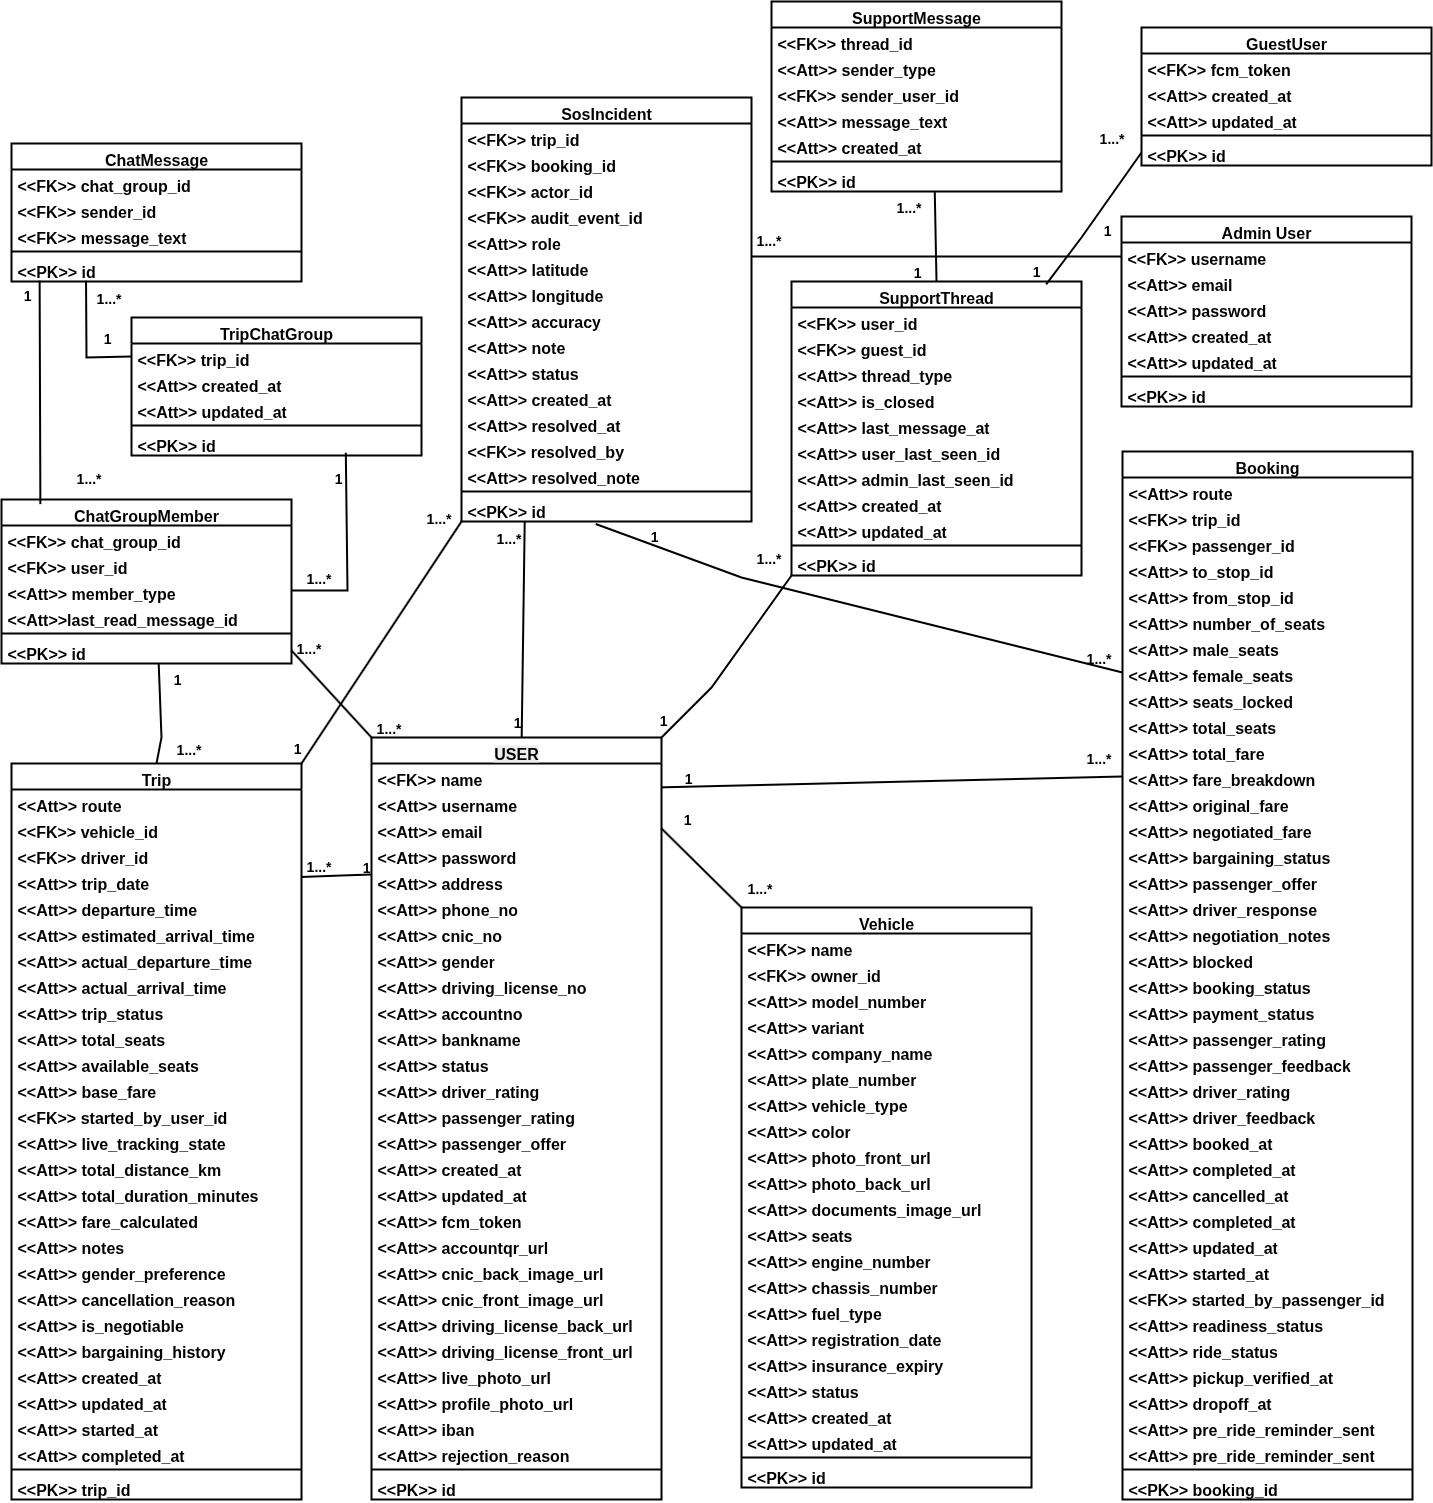
\includegraphics[width=0.9\textwidth,keepaspectratio,height=0.8\textheight]{assets/db_diagrams/DB_SCHEM.png}
\caption{Physical Database Schema Diagram showing table structures and relationships}
\label{fig:schema}
\end{figure}

The database schema is normalized to 3NF to eliminate Data redundancy. This structured design ensures \textbf{data integrity} by enforcing strict relational constraints (Foreign Keys) between tables like Users, Rides, and Bookings. It supports \textbf{efficient querying} through indexing on frequently accessed fields like \texttt{user\_id} and \texttt{ride\_id}. The schema's modularity allows \textbf{scalability} by enabling seamless extension of tables without affecting core operations. Finally, \textbf{security} is maintained by isolating sensitive authentication data in the core User table away from public operational data.

\subsection{Data Dictionary}

The Data Dictionary defines the structure of all primary data elements in the database.

\textbf{Guidelines:}
\begin{itemize}
    \item Include field name, Data type, Size, Description, Constraints.
\end{itemize}

\begin{table}[H]
\centering
\caption{Data Dictionary – Booking Table}
\renewcommand{\arraystretch}{1.5}
\begin{tabular}{|p{3cm}|p{3cm}|p{7cm}|}
\hline
\textbf{Attribute} & \textbf{Type} & \textbf{Description} \\
\hline
booking\_id & CharField & Unique booking identifier (PK) \\
\hline
trip & ForeignKey & Associated Trip (FK to Trip) \\
\hline
passenger & ForeignKey & Associated Passenger (FK to UsersData) \\
\hline
from\_stop & ForeignKey & Pickup stop (FK to RouteStop) \\
\hline
to\_stop & ForeignKey & Drop-off stop (FK to RouteStop) \\
\hline
number\_of\_seats & Integer & Total seats booked for this request \\
\hline
male\_seats & Integer & Number of seats for male passengers \\
\hline
female\_seats & Integer & Number of seats for female passengers \\
\hline
total\_fare & Integer & Total fare for the booking \\
\hline
booking\_status & CharField & Current status (PENDING, CONFIRMED, etc.) \\
\hline
payment\_status & CharField & Payment status (PENDING, COMPLETED, etc.) \\
\hline
\end{tabular}
\end{table}

\begin{table}[H]
\centering
\caption{Data Dictionary – ChatMessage Table}
\renewcommand{\arraystretch}{1.5}
\begin{tabular}{|p{3cm}|p{3cm}|p{7cm}|}
\hline
\textbf{Attribute} & \textbf{Type} & \textbf{Description} \\
\hline
id & AutoField & Unique message identifier (PK) \\
\hline
chat\_group & ForeignKey & Associated chat group (FK to TripChatGroup) \\
\hline
sender & ForeignKey & User who sent the message (FK to UsersData) \\
\hline
message\_type & CharField & Type of message (TEXT, IMAGE, SYSTEM) \\
\hline
message\_text & TextField & Content of the message \\
\hline
created\_at & DateTime & Timestamp when message was sent \\
\hline
is\_deleted & Boolean & Flag for deleted messages \\
\hline
\end{tabular}
\end{table}

\begin{table}[H]
\centering
\caption{Data Dictionary – SosIncident Table}
\renewcommand{\arraystretch}{1.5}
\begin{tabular}{|p{3cm}|p{3cm}|p{7cm}|}
\hline
\textbf{Attribute} & \textbf{Type} & \textbf{Description} \\
\hline
id & AutoField & Unique incident identifier (PK) \\
\hline
trip & ForeignKey & Associated trip (FK to Trip) \\
\hline
actor & ForeignKey & Person who triggered SOS (FK to UsersData) \\
\hline
role & CharField & Role of the actor (Passenger/Driver) \\
\hline
latitude & Decimal & GPS latitude at trigger time \\
\hline
longitude & Decimal & GPS longitude at trigger time \\
\hline
status & CharField & Current status (OPEN, RESOLVED) \\
\hline
created\_at & DateTime & Time incident was recorded \\
\hline
\end{tabular}
\end{table}

\begin{table}[H]
\centering
\caption{Data Dictionary – Driver Fields in UsersData}
\renewcommand{\arraystretch}{1.5}
\begin{tabular}{|p{3cm}|p{3cm}|p{7cm}|}
\hline
\textbf{Attribute} & \textbf{Type} & \textbf{Description} \\
\hline
driving\_license\_no & CharField & National driving license identification \\
\hline
driving\_license\_front\_url & URLField & Link to license front image \\
\hline
driving\_license\_back\_url & URLField & Link to license back image \\
\hline
driver\_rating & Decimal & Average rating as a driver \\
\hline
status & CharField & Verification status (PENDING, VERIFIED) \\
\hline
bankname & CharField & Name of driver's bank for payments \\
\hline
iban & CharField & Bank account IBAN for transfers \\
\hline
\end{tabular}
\end{table}

\begin{table}[H]
\centering
\caption{Data Dictionary – TripLiveLocationUpdate Table}
\renewcommand{\arraystretch}{1.5}
\begin{tabular}{|p{3cm}|p{3cm}|p{7cm}|}
\hline
\textbf{Attribute} & \textbf{Type} & \textbf{Description} \\
\hline
trip & ForeignKey & Associated trip (FK to Trip) \\
\hline
user & ForeignKey & User providing update (FK to UsersData) \\
\hline
latitude & Decimal & Current latitude coordinate \\
\hline
longitude & Decimal & Current longitude coordinate \\
\hline
speed\_mps & Float & Speed in meters per second \\
\hline
recorded\_at & DateTime & Timestamp of the location update \\
\hline
\end{tabular}
\end{table}

\begin{table}[H]
\centering
\caption{Data Dictionary – Passenger Fields in UsersData}
\renewcommand{\arraystretch}{1.5}
\begin{tabular}{|p{3cm}|p{3cm}|p{7cm}|}
\hline
\textbf{Attribute} & \textbf{Type} & \textbf{Description} \\
\hline
passenger\_rating & Decimal & Average rating as a passenger \\
\hline
fcm\_token & TextField & Push notification token \\
\hline
address & TextField & Primary residence address \\
\hline
phone\_no & CharField & Contact number \\
\hline
name & CharField & Full legal name \\
\hline
\end{tabular}
\end{table}

\begin{table}[H]
\centering
\caption{Data Dictionary – TripPayment Table}
\renewcommand{\arraystretch}{1.5}
\begin{tabular}{|p{3cm}|p{3cm}|p{7cm}|}
\hline
\textbf{Attribute} & \textbf{Type} & \textbf{Description} \\
\hline
booking & ForeignKey & Associated booking (FK to Booking) \\
\hline
payment\_method & CharField & Method (CASH, BANK\_TRANSFER, etc.) \\
\hline
amount & Integer & Payment amount paid in PKR \\
\hline
transaction\_id & CharField & Unique external transaction reference \\
\hline
payment\_status & CharField & Status (PENDING, COMPLETED, FAILED) \\
\hline
created\_at & DateTime & Time when payment was initiated \\
\hline
\end{tabular}
\end{table}

\begin{table}[H]
\centering
\caption{Data Dictionary – Trip Table}
\renewcommand{\arraystretch}{1.5}
\begin{tabular}{|p{3cm}|p{3cm}|p{7cm}|}
\hline
\textbf{Attribute} & \textbf{Type} & \textbf{Description} \\
\hline
trip\_id & CharField & Unique trip identifier (PK) \\
\hline
route & ForeignKey & Associated route (FK to Route) \\
\hline
vehicle & ForeignKey & Assigned vehicle (FK to Vehicle) \\
\hline
driver & ForeignKey & Assigned driver (FK to UsersData) \\
\hline
trip\_date & DateField & Date of the scheduled trip \\
\hline
departure\_time & TimeField & Scheduled start time \\
\hline
trip\_status & CharField & Status (SCHEDULED, IN\_PROGRESS, etc.) \\
\hline
available\_seats & Integer & Remaining seats for booking \\
\hline
base\_fare & Integer & Standard fare for the trip \\
\hline
\end{tabular}
\end{table}

\begin{table}[H]
\centering
\caption{Data Dictionary – Route Table}
\renewcommand{\arraystretch}{1.5}
\begin{tabular}{|p{3cm}|p{3cm}|p{7cm}|}
\hline
\textbf{Attribute} & \textbf{Type} & \textbf{Description} \\
\hline
route\_id & CharField & Unique route code (e.g., R001) (PK) \\
\hline
route\_name & CharField & Descriptive name for the route \\
\hline
total\_distance\_km & Decimal & Total length of the route \\
\hline
estimated\_duration & Integer & Estimated travel time in minutes \\
\hline
route\_geometry & JSONField & List of GPS points for map rendering \\
\hline
is\_active & Boolean & Whether the route is currently operational \\
\hline
\end{tabular}
\end{table}

\begin{table}[H]
\centering
\caption{Data Dictionary – EmergencyContact Table}
\renewcommand{\arraystretch}{1.5}
\begin{tabular}{|p{3cm}|p{3cm}|p{7cm}|}
\hline
\textbf{Attribute} & \textbf{Type} & \textbf{Description} \\
\hline
user & OneToOneField & Associated user (FK to UsersData) \\
\hline
name & CharField & Contact person's name \\
\hline
relation & CharField & Relationship to user (e.g., Father, Friend) \\
\hline
phone\_no & CharField & Emergency contact phone number \\
\hline
email & EmailField & Emergency contact email address \\
\hline
\end{tabular}
\end{table}

\begin{table}[H]
\centering
\caption{Data Dictionary – UsersData Table}
\renewcommand{\arraystretch}{1.5}
\begin{tabular}{|p{3cm}|p{3.5cm}|p{6.5cm}|}
\hline
\textbf{Attribute} & \textbf{Type} & \textbf{Description} \\
\hline
id & AutoField & Unique user record ID (PK) \\
\hline
username & CharField & Unique login username \\
\hline
email & EmailField & Unique registered email address \\
\hline
password & CharField & Hashed password string \\
\hline
cnic\_no & CharField & Identity card number (XXXXX-XXXXXXX-X) \\
\hline
gender & CharField & male, female \\
\hline
status & CharField & PENDING, VERIFIED, BANNED \\
\hline
created\_at & DateTime & Signup timestamp \\
\hline
\end{tabular}
\end{table}

\begin{table}[H]
\centering
\caption{Data Dictionary – Vehicle Table}
\renewcommand{\arraystretch}{1.5}
\begin{tabular}{|p{3cm}|p{3cm}|p{7cm}|}
\hline
\textbf{Attribute} & \textbf{Type} & \textbf{Description} \\
\hline
id & AutoField & Unique vehicle identifier (PK) \\
\hline
owner & ForeignKey & Driver owning vehicle (FK to UsersData) \\
\hline
model\_number & CharField & Vehicle model (e.g., Corolla 2022) \\
\hline
plate\_number & CharField & Unique license plate number \\
\hline
vehicle\_type & CharField & TW (Two Wheeler), FW (Four Wheeler) \\
\hline
seats & Integer & Number of passenger seats \\
\hline
fuel\_type & CharField & Petrol, Diesel, CNG, etc. \\
\hline
status & CharField & VERIFIED, PENDING, REJECTED \\
\hline
\end{tabular}
\end{table}

\begin{table}[H]
\centering
\caption{Data Dictionary – RouteStop Table}
\renewcommand{\arraystretch}{1.5}
\begin{tabular}{|p{3cm}|p{3cm}|p{7cm}|}
\hline
\textbf{Attribute} & \textbf{Type} & \textbf{Description} \\
\hline
route & ForeignKey & Parent route (FK to Route) \\
\hline
stop\_name & CharField & Name of the stop/pickup point \\
\hline
stop\_order & Integer & Sequence of the stop in the route \\
\hline
latitude & Decimal & GPS latitude for the stop \\
\hline
longitude & Decimal & GPS longitude for the stop \\
\hline
address & TextField & Detailed address of the stop \\
\hline
\end{tabular}
\end{table}

%===========================================================
\section{Database Tables / Collections}
%===========================================================

This section describes the logical database design of the system. It presents the major relational tables (for SQL-based systems) or collections (for NoSQL-based systems). The database structure is designed to ensure data consistency, integrity, security, and scalability.

Each table or collection includes primary keys, relationships, and major attributes relevant to system functionality.

\subsection{User Collection / Table}

The User table stores authentication credentials and user profile information. It supports role-based access control and secure authentication.

\textbf{Description:}
\begin{itemize}
    \item \textbf{Primary Key:} user\_id
    \item \textbf{Relationships:} Linked to transactions, predictions, or system logs.
    \item \textbf{Authentication Attributes:} Email, password hash, role, account status.
\end{itemize}

\begin{table}[H]
\centering
\caption{UsersData Table Structure}
\renewcommand{\arraystretch}{1.5}
\begin{tabular}{|p{3cm}|p{3.5cm}|p{3cm}|p{5cm}|}
\hline
\textbf{Field Name} & \textbf{Data Type} & \textbf{Constraint} & \textbf{Description} \\
\hline
id & AutoField & Primary Key & Unique identifier for each user \\
\hline
name & VARCHAR(100) & Not Null & User's full name \\
\hline
username & VARCHAR(100) & Unique, Not Null & Unique login username \\
\hline
email & EmailField & Unique, Not Null & Registered email address \\
\hline
password & VARCHAR(128) & MinLength(8) & Hashed password string \\
\hline
cnic\_no & VARCHAR(15) & Unique, Regex & Identity card number \\
\hline
status & VARCHAR(10) & Choice & Enum: PENDING, VERIFIED, BANNED \\
\hline
\end{tabular}
\end{table}

\subsection{Core Data Collection}

This subsection describes domain-specific core data tables. These structures store the primary operational data processed by the Ride Booking system.

\textbf{Domain-Specific Tables:}

\subsubsection{Passenger Data (UsersData)}
\begin{table}[H]
\centering
\caption{Passenger-Specific Table Fields}
\renewcommand{\arraystretch}{1.5}
\begin{tabular}{|p{3cm}|p{3.5cm}|p{7cm}|}
\hline
\textbf{Field Name} & \textbf{Data Type} & \textbf{Description} \\
\hline
passenger\_rating & DecimalField & Average rating from drivers \\
\hline
address & TextField & Pickup/Home address \\
\hline
phone\_no & CharField & Contact number with validation \\
\hline
fcm\_token & TextField & Firebase notification token \\
\hline
\end{tabular}
\end{table}

\subsubsection{Driver Data (UsersData)}
\begin{table}[H]
\centering
\caption{Driver-Specific Table Fields}
\renewcommand{\arraystretch}{1.5}
\begin{tabular}{|p{3cm}|p{3.5cm}|p{7cm}|}
\hline
\textbf{Field Name} & \textbf{Data Type} & \textbf{Description} \\
\hline
driving\_license\_no & CharField & Professional license number \\
\hline
driving\_license\_front\_url & URLField & Image of license front \\
\hline
bankname & CharField & Transaction bank name \\
\hline
iban & CharField & International Bank Account Number \\
\hline
driver\_rating & DecimalField & Average rating from passengers \\
\hline
\end{tabular}
\end{table}

\subsubsection{Vehicle Table}
\begin{table}[H]
\centering
\caption{Vehicle Table}
\renewcommand{\arraystretch}{1.5}
\begin{tabular}{|p{3cm}|p{3.5cm}|p{7cm}|}
\hline
\textbf{Field Name} & \textbf{Data Type} & \textbf{Description} \\
\hline
id (PK) & AutoField & Unique database ID \\
\hline
owner (FK) & ForeignKey & Link to UsersData (Owner) \\
\hline
model\_number & CharField & Vehicle specific model \\
\hline
plate\_number & CharField & UNIQUE registration plate \\
\hline
vehicle\_type & CharField & Choices: TW or FW \\
\hline
seats & PositiveInt & Available seating capacity \\
\hline
fuel\_type & CharField & Petrol, Diesel, CNG, etc. \\
\hline
\end{tabular}
\end{table}

\subsubsection{Route Table}
\begin{table}[H]
\centering
\caption{Route Table}
\renewcommand{\arraystretch}{1.5}
\begin{tabular}{|p{3cm}|p{3.5cm}|p{7cm}|}
\hline
\textbf{Field Name} & \textbf{Data Type} & \textbf{Description} \\
\hline
route\_id & CharField & Unique identifier (e.g., R001) \\
\hline
route\_name & CharField & Name of the route \\
\hline
total\_distance\_km & DecimalField & Length of trip in km \\
\hline
estimated\_duration & IntegerField & Duration in minutes \\
\hline
route\_geometry & JSONField & Polylines for map display \\
\hline
is\_active & BooleanField & Status of the route \\
\hline
\end{tabular}
\end{table}

\subsubsection{Booking Table}
\begin{table}[H]
\centering
\caption{Booking Table}
\renewcommand{\arraystretch}{1.5}
\begin{tabular}{|p{3cm}|p{3.5cm}|p{7cm}|}
\hline
\textbf{Field Name} & \textbf{Data Type} & \textbf{Description} \\
\hline
booking\_id (PK) & CharField & Unique Booking identifier \\
\hline
trip (FK) & ForeignKey & Link to Trip record \\
\hline
passenger (FK) & ForeignKey & Link to UsersData record \\
\hline
number\_of\_seats & IntegerField & Seats requested \\
\hline
total\_fare & IntegerField & Final calculated cost \\
\hline
booking\_status & CharField & PENDING, CONFIRMED, etc. \\
\hline
payment\_status & CharField & Payment state \\
\hline
\end{tabular}
\end{table}

\subsubsection{Trip Table}
\begin{table}[H]
\centering
\caption{Trip Table}
\renewcommand{\arraystretch}{1.5}
\begin{tabular}{|p{3cm}|p{3.5cm}|p{7cm}|}
\hline
\textbf{Field Name} & \textbf{Data Type} & \textbf{Description} \\
\hline
trip\_id (PK) & CharField & Unique Trip identifier \\
\hline
route (FK) & ForeignKey & FK to Route model \\
\hline
vehicle (FK) & ForeignKey & FK to Vehicle model \\
\hline
driver (FK) & ForeignKey & FK to UsersData model \\
\hline
trip\_date & DateField & Date of travel \\
\hline
trip\_status & CharField & SCHEDULED, COMPLETED, etc. \\
\hline
available\_seats & IntegerField & Current capacity left \\
\hline
\end{tabular}
\end{table}

\subsubsection{TripPayment Table}
\begin{table}[H]
\centering
\caption{TripPayment Table}
\renewcommand{\arraystretch}{1.5}
\begin{tabular}{|p{3cm}|p{3.5cm}|p{7cm}|}
\hline
\textbf{Field Name} & \textbf{Data Type} & \textbf{Description} \\
\hline
id (PK) & AutoField & Unique Payment ID \\
\hline
booking (FK) & ForeignKey & FK to Booking model \\
\hline
payment\_method & CharField & CASH, BANK\_TRANSFER, etc. \\
\hline
amount & IntegerField & Fare amount in PKR \\
\hline
payment\_status & CharField & PENDING, COMPLETED, etc. \\
\hline
created\_at & DateTimeField & Initial timestamp \\
\hline
\end{tabular}
\end{table}

\subsubsection{SosIncident Table}
\begin{table}[H]
\centering
\caption{SosIncident Table}
\renewcommand{\arraystretch}{1.5}
\begin{tabular}{|p{3cm}|p{3.5cm}|p{7cm}|}
\hline
\textbf{Field Name} & \textbf{Data Type} & \textbf{Description} \\
\hline
id (PK) & AutoField & Unique SOS entry \\
\hline
trip (FK) & ForeignKey & FK to Trip model \\
\hline
actor (FK) & ForeignKey & Link to triggering User \\
\hline
role & CharField & Role (Passenger/Driver) \\
\hline
status & CharField & OPEN or RESOLVED \\
\hline
created\_at & DateTimeField & Time of trigger \\
\hline
\end{tabular}
\end{table}

\subsubsection{EmergencyContact Table}
\begin{table}[H]
\centering
\caption{EmergencyContact Table}
\renewcommand{\arraystretch}{1.5}
\begin{tabular}{|p{3cm}|p{3.5cm}|p{7cm}|}
\hline
\textbf{Field Name} & \textbf{Data Type} & \textbf{Description} \\
\hline
user (FK) & OneToOneField & Link to UsersData \\
\hline
name & CharField & Contact name \\
\hline
phone\_no & CharField & Verified contact number \\
\hline
relation & CharField & Relationship to user \\
\hline
\end{tabular}
\end{table}

\subsubsection{ChatMessage Table}
\begin{table}[H]
\centering
\caption{ChatMessage Table}
\renewcommand{\arraystretch}{1.5}
\begin{tabular}{|p{3cm}|p{3.5cm}|p{7cm}|}
\hline
\textbf{Field Name} & \textbf{Data Type} & \textbf{Description} \\
\hline
id (PK) & AutoField & Message primary key \\
\hline
chat\_group (FK) & ForeignKey & FK to TripChatGroup \\
\hline
sender (FK) & ForeignKey & FK to UsersData \\
\hline
message\_type & CharField & TEXT, IMAGE, SYSTEM \\
\hline
message\_text & TextField & Encrypted text content \\
\hline
\end{tabular}
\end{table}

\subsection{Relationships Between Tables}

Database relationships define how data entities are connected within the Lets Go Ride Sharing App system.

\begin{itemize}
    \item \textbf{One Driver $\rightarrow$ Many Vehicles} (1-to-M)
    \item \textbf{One Passenger $\rightarrow$ Many Bookings} (1-to-M)
    \item \textbf{Many Bookings $\rightarrow$ One Trip} (M-to-1)
    \item \textbf{One Booking $\rightarrow$ One Payment} (1-to-1)
    \item \textbf{One Trip $\rightarrow$ Many SosIncidents} (1-to-M)
    \item \textbf{One User $\rightarrow$ One EmergencyContact} (1-to-1)
    \item \textbf{One Trip $\rightarrow$ One ChatGroup} (1-to-1)
    \item \textbf{One ChatGroup $\rightarrow$ Many ChatMessages} (1-to-M)
\end{itemize}

An Entity-Relationship (ER) Diagram visually represents these relationships.

\subsection{Security and Data Integrity}

To ensure confidentiality and integrity of stored data, the following measures are implemented:
\begin{itemize}
    \item \textbf{Password Encryption} using secure hashing algorithms (e.g., bcrypt, SHA-256 with salt).
    \item \textbf{Role-Based Access Control (RBAC)} to restrict unauthorized access between passengers, drivers, and admins.
    \item \textbf{Input validation} and constraint enforcement at the database level (e.g., NOT NULL, UNIQUE constraints).
    \item \textbf{Secure communication} using HTTPS for API endpoints accessing the DB.
    \item \textbf{Regular database backup} and disaster recovery strategy.
\end{itemize}

\subsection{Scalability Considerations}

The database design incorporates scalability mechanisms to support future growth of the ride-sharing platform.
\begin{itemize}
    \item \textbf{Horizontal Scaling} using distributed database systems.
    \item \textbf{Indexing} on frequently queried attributes (like \texttt{pickup\_location}, \texttt{drop\_location}, \texttt{status}) to improve search performance.
    \item \textbf{Caching strategies} for frequently accessed data like active ride and booking summaries.
    \item \textbf{Load balancing} across database instances for API request handling.
    \item \textbf{Partitioning or sharding} for large-scale data environments (e.g., partitioning old ride records by year).
\end{itemize}

%===========================================================
\section{Chapter Summary}
%===========================================================

This chapter discussed the software architecture and design of the Let’s Go system in detail. It outlined the transition from requirements to an actual system blueprint using an Agile incremental model. 

Key modeling diagrams—including Activity, Class, Sequence, and State Transition diagrams—were presented to illustrate the dynamic and structural behavior of the system. Data Flow Diagrams (DFDs) detailed the movement of data across various operational phases, from authentication to ride tracking and dispute resolution. 

The chapter concluded with a comprehensive data design section, explicitly defining PostgreSQL schemas, ER diagrams, data dictionaries, and database relationships to ensure a scalable, secure, and normalized data architecture.